%%%%%%%%%%%%%%%%%%%%%%%%%%%%%%%%%%%%%%%%%%%%%%%%%%%%%%%%%%%%%%%%%%%%%
%%                                                                 %%
%% Please do not use \input{...} to include other tex files.       %%
%% Submit your LaTeX manuscript as one .tex document.              %%
%%                                                                 %%
%% All additional figures and files should be attached             %%
%% separately and not embedded in the \TeX\ document itself.       %%
%%                                                                 %%
%%%%%%%%%%%%%%%%%%%%%%%%%%%%%%%%%%%%%%%%%%%%%%%%%%%%%%%%%%%%%%%%%%%%%

%%\documentclass[referee,sn-basic]{sn-jnl}% referee option is meant for double line spacing

%%=======================================================%%
%% to print line numbers in the margin use lineno option %%
%%=======================================================%%

%%\documentclass[lineno,sn-basic]{sn-jnl}% Basic Springer Nature Reference Style/Chemistry Reference Style

%%======================================================%%
%% to compile with pdflatex/xelatex use pdflatex option %%
%%======================================================%%

%%\documentclass[pdflatex,sn-basic]{sn-jnl}% Basic Springer Nature Reference Style/Chemistry Reference Style

%%\documentclass[sn-basic]{sn-jnl}% Basic Springer Nature Reference Style/Chemistry Reference Style
\documentclass[sn-mathphys,Numbered]{sn-jnl}% Math and Physical Sciences Reference Style
%%\documentclass[sn-aps]{sn-jnl}% American Physical Society (APS) Reference Style
%%\documentclass[sn-vancouver]{sn-jnl}% Vancouver Reference Style
%%\documentclass[sn-apa]{sn-jnl}% APA Reference Style
%%\documentclass[sn-chicago]{sn-jnl}% Chicago-based Humanities Reference Style
%%\documentclass[sn-standardnature]{sn-jnl}% Standard Nature Portfolio Reference Style
%%\documentclass[default]{sn-jnl}% Default
%%\documentclass[default,iicol]{sn-jnl}% Default with double column layout

%%%% Standard Packages
%%<additional latex packages if required can be included here>
%%%%

%%%%%=============================================================================%%%%
%%%%  Remarks: This template is provided to aid authors with the preparation
%%%%  of original research articles intended for submission to journals published 
%%%%  by Springer Nature. The guidance has been prepared in partnership with 
%%%%  production teams to conform to Springer Nature technical requirements. 
%%%%  Editorial and presentation requirements differ among journal portfolios and 
%%%%  research disciplines. You may find sections in this template are irrelevant 
%%%%  to your work and are empowered to omit any such section if allowed by the 
%%%%  journal you intend to submit to. The submission guidelines and policies 
%%%%  of the journal take precedence. A detailed User Manual is available in the 
%%%%  template package for technical guidance.
%%%%%=============================================================================%%%%

\jyear{2021}%

%% as per the requirement new theorem styles can be included as shown below
\theoremstyle{thmstyleone}%
\newtheorem{theorem}{Theorem}%  meant for continuous numbers
%%\newtheorem{theorem}{Theorem}[section]% meant for sectionwise numbers
%% optional argument [theorem] produces theorem numbering sequence instead of independent numbers for Proposition
\newtheorem{proposition}[theorem]{Proposition}% 
%%\newtheorem{proposition}{Proposition}% to get separate numbers for theorem and proposition etc.

\theoremstyle{thmstyletwo}%
\newtheorem{example}{Example}%
\newtheorem{remark}{Remark}%

\theoremstyle{thmstylethree}%
\newtheorem{definition}{Definition}%

\raggedbottom
%%\unnumbered% uncomment this for unnumbered level heads

%% My used library
\usepackage{enumitem}
\usepackage[numbers]{natbib}
%\usepackage{notoccite}
\usepackage{subcaption}
\usepackage{amsmath,amssymb}
\usepackage{graphicx, adjustbox}
\usepackage{caption}
\usepackage{longtable,booktabs,array}
\usepackage{csquotes}
\usepackage{multirow} % Required for multirows
\usepackage{longtable,booktabs,array}
\usepackage{calc} % for calculating minipage widths
%\graphicspath{{Figs}{Figs/}}

\begin{document}

\title[Article Title]{English Textbook Content Comprehension with LDA for the perspective of Bangladesh}

%%=============================================================%%
%% Prefix	-> \pfx{Dr}
%% GivenName	-> \fnm{Joergen W.}
%% Particle	-> \spfx{van der} -> surname prefix
%% FamilyName	-> \sur{Ploeg}
%% Suffix	-> \sfx{IV}
%% NatureName	-> \tanm{Poet Laureate} -> Title after name
%% Degrees	-> \dgr{MSc, PhD}
%% \author*[1,2]{\pfx{Dr} \fnm{Joergen W.} \spfx{van der} \sur{Ploeg} \sfx{IV} \tanm{Poet Laureate} 
%%                 \dgr{MSc, PhD}}\email{iauthor@gmail.com}
%%=============================================================%%



%\affil[2]{\orgdiv{Department}, \orgname{Organization}, \orgaddress{\street{Street}, \city{City}, \postcode{10587}, \state{State}, \country{Country}}}
%
%\affil[3]{\orgdiv{Department}, \orgname{Organization}, \orgaddress{\street{Street}, \city{City}, \postcode{610101}, \state{State}, \country{Country}}}

%%==================================%%
%% sample for unstructured abstract %%
%%==================================%%

\abstract{
In Bangladesh, rural students exhibit inadequate proficiency in English language. Pupils can not fully grasp context from National Curriculum and Textbook Board (NCTB) provided textbooks. In this research study an unsupervised topic modeling LDA approach is proposed to comprehend the context of NCTB's English book. Exploratory analysis is shown to depict significant keywords related to subtle topic in context. It identifies latent topics within lessons that uncovers coherent themes from textual data. Extensive analysis is conducted to visualize, high impact keywords, co-occurrence patterns and correlation between extracted topics. It is anticipated it improves curriculum provided English textbook content synthesis and acquisition skill of learners. A prototype mobile app is developed which incorporates topic modeling extracted keywords. Furthermore, qualitative research survey is undertaken to evaluate its effectiveness on end-users (course instructors of Bangladesh\textquotesingle s higher secondary school). The challenges, future potential of LDA extracted content integrated mobile app into the learning process is explored. After collecting feedback, word clouds were used to analyze the participants\textquotesingle{} recommended terms, and the LIWC approach is used to estimate overall sentiment. LIWC score showed positive sentiment and survey process enticed the participants, demonstrates learners eager to use NLP technology driven topic modeling approach in teaching and learning, and
there are tremendous opportunities.}



%%================================%%
%% Sample for structured abstract %%
%%================================%%

% \abstract{\textbf{Purpose:} The abstract serves both as a general introduction to the topic and as a brief, non-technical summary of the main results and their implications. The abstract must not include subheadings (unless expressly permitted in the journal's Instructions to Authors), equations or citations. As a guide the abstract should not exceed 200 words. Most journals do not set a hard limit however authors are advised to check the author instructions for the journal they are submitting to.
% 
% \textbf{Methods:} The abstract serves both as a general introduction to the topic and as a brief, non-technical summary of the main results and their implications. The abstract must not include subheadings (unless expressly permitted in the journal's Instructions to Authors), equations or citations. As a guide the abstract should not exceed 200 words. Most journals do not set a hard limit however authors are advised to check the author instructions for the journal they are submitting to.
% 
% \textbf{Results:} The abstract serves both as a general introduction to the topic and as a brief, non-technical summary of the main results and their implications. The abstract must not include subheadings (unless expressly permitted in the journal's Instructions to Authors), equations or citations. As a guide the abstract should not exceed 200 words. Most journals do not set a hard limit however authors are advised to check the author instructions for the journal they are submitting to.
% 
% \textbf{Conclusion:} The abstract serves both as a general introduction to the topic and as a brief, non-technical summary of the main results and their implications. The abstract must not include subheadings (unless expressly permitted in the journal's Instructions to Authors), equations or citations. As a guide the abstract should not exceed 200 words. Most journals do not set a hard limit however authors are advised to check the author instructions for the journal they are submitting to.}

\keywords{Natural Language Processing (NLP), Topic Modeling, Latent Dirichlet Allocation (LDA), Exploratory Analysis, Textbook Learning, Coherence}

%%\pacs[JEL Classification]{D8, H51}

%%\pacs[MSC Classification]{35A01, 65L10, 65L12, 65L20, 65L70}

\maketitle

\section{Introduction}\label{sec1}
In Bangladesh there is lacking in effective acquisition, synthesis skill of English language from National Curriculum and Textbook Board (NCTB) curriculum provided textbook \cite{report_schools_2018, statistics_bangladesh_2017}. Specially in the rural area in National Board examinations like SSC, HSC most of the student get poor marks in English subject \cite{noauthor_bangladesh_2021, habib_english_2018}. It is anticipated students have lacking in understanding context. Topic modeling can play a significant role for context understanding for curriculum provided English textbook \cite{qiang2020short, bethard_topic_2009, ali_transportation_2019, slater_using_2017, guerra_when_2013}. Topic modeling is machine learning technique of Natural Language Processing field, offers a promising unsupervised approach to identify latent topics within provided documents \cite{jelodar_latent_2019, gupta_pan_lda_2021, pichardo_lagunas_svd_lda_2015, selvi_classification_2019, pichardo_lagunas_svd_lda_2015_1}. It can help identify the main themes, concepts, and topics within the textbook\textquotesingle s content, enabling instructors to tailor the learning experience to individual students. LDA is one the prominent algorithm which can be used for topic modeling \cite{blei2003latent}. It provides coherent topics, dominant keywords, latent combination of features that characterizes similarities between topics. In this research LDA extracted keywords are rearranged and incorporated into a mobile app to observe user experience. 

Across all English learning applications via digital media, about 55\% exercise activities involved vocabulary learning \cite{klimova_evaluation_2018, hao_evaluative_2019, polakova_mobile_2019} and other exercises includes quizzes, flash cards, and games \cite{xu_scoping_2020, shortt_gamification_2023} for enhancing learners' comprehension and self-checks ability \cite{bernacki_mobile_2020, metruk_use_2021, isamiddinovna_mobile_2019, klimova_evaluation_2018}. Therefore, it can be assumed that if LDA extracted vocabulary is learned then it will improve contextual understanding, enhance synthesis knowledge of subtle meaning of correlated topics. There are numerous English learning apps are prevailing \cite{metruk_use_2021, rafiq_sustaining_2021, chen_evaluating_2016}. One caveat is of these apps are very few of them are based on Curriculum Board provided Textbook for learning English hence, could not able to attract a large number of pupils in Bangladesh who are mostly depended on NCBI textbook.  To grasp the English language knowledge from curriculum provided textbook a novel approach Latent Dirichlet Allocation (LDA) based unsupervised Topic modeling using textbook corpus is adopted and exploratory analysis is demonstrated in this study. Our anticipation is through this way student can able to interpret meaningful information facilitates students to understand the correlated topics and important keywords related to that topics leads to understand the subtle meaning of the textbook context.

\subsection{Research Overview} 
To detect underlying themes or topics keywords within a Textbook corpus an unsupervised probabilistic topic modeling technique LDA is used in this research \cite{jelodar_latent_2019} (see section \ref{lda_mdel} for details). Topic modeling of LDA doesn\textquotesingle t directly account for student engagement such as learning tasks in mobile apps \cite{sandberg_mobile_2011}. Hence a prototype app is developed and qualitative survey is conducted to observe the instructor\textquotesingle s sentiment impact similar to research paper in \cite{oz2015investigation}. Qualitative survey research is undertaken to evaluate the effectiveness of unsupervised topic modeling LDA Bangladesh\textquotesingle s National Curriculum Textbook Board (NCTB) provided English Textbook for Higher secondary school education. This study seeks to ascertain if instructors can teach and students can learn English better if a mobile app is introduced which includes NLP\textquotesingle s LDA driven topic modeling applied extracted keywords and analysis. A prototype mobile app is developed to incorporate the topic modeling extracted keywords into the app. This article presents the key findings and insights from the survey, shedding light on the prospective of learners especially instructors. In the survey questions, it was indicated whether the students, teachers/instructors would find it acceptable and appreciated if textbook information were made available through a mobile app and presented in interactive format. To demonstrate the mobile app idea during the interrogation survey session a prototype is also prepared. Participants were asked for suggestions on how to make the app better and about any shortcomings. After collecting feedback, word clouds were used (see \ref{wordcloud}) to analyze the frequency of the participants\textquotesingle{} recommended terms, and the LIWC approach was used to estimate overall sentiment (see \ref{liwc}). The main contributions of this research study are:
\begin{itemize}
\item Unsupervised topic modeling technique LDA based keyword extraction from textbooks for the Bangladeshi setting affects the efficacy of education.
\item Along with theoretical analysis with LDA a prototype demonstration qualitative survey conducted to realize its potential and credibility
\item English Textbook content comprehension facilitates empowerment via education of mass population has direct impact on sustainability
\end{itemize}
\hfill
The following sections are organized as follows. Background literature studied in section \ref{lit_review} illustrates LDA for dominant keywords determination, followed by methodology. Survey response visualization and analysis depicted in (subsection \ref{vis_part}). Following section \ref{exp_analysis} demonstrated the experiments and contains analysis separated into several subsections (\ref{coh_measure}, \ref{dom_topic} and \ref{top_term_vis}). Then results discussion, limitations and conclusion are illustrated in section \ref{res_dis}, \ref{limitat} and \ref{conclu} respectively. 

  
\section{Literature Review}\label{lit_review}

Topic modeling has been used for semantic search, ontology exploration, classification, dominant keywords searching in many research studies. For curriculum based textbook study it could be an option is not revealed from rigorous search in online repositories, which we addressed in this research study. This research model is infusing Textbook features into LDA based topic modeling to discover a set of topic-words from the provided document for Textbook comprehension and understanding context. Similar approaches and implications are described below:

\subsection{Textbook Content extraction with LDA}\label{Text_content_lda}
According to Krishna Raj \cite{raj_p_m_sentiment_2022} the human brain has a propensity to forget a number of facts regarding the events in book. The LDA model can able to scan through large quantities of text in the book and extract intriguing key concepts terms. Thereby, a book can be adapted by learners with the help of the LDA model, greatly refine the learning process. Similar approch proposed by  Rani et al. for Hindi books and stories, a topic modeling text summarizing approach proposed in 2021 \cite{rani_extractive_2021}. By incorporating linguistic features into LDA-based topic modeling, the suggested model is can find a set of topic-words from the given material to understand context.  Educational content-based topic modeling for an Intelligent system to develop a tutoring system is proposed in \cite{slater_using_2017} by researcher Stefan Slater in 2017. To understand the linguistic content of mathematical problems, a personalized learning system is suggested that makes use of correlated topic modeling of natural language processing, an approach which can extract important keywords. A variety of significant and useful contents are explored in the context of addressing mathematical difficulties. They demonstrated that topic modeling is a useful method for a personalized learning systems. For key terms detection within articles LDA based topic modeling has been used in many research studies in which dominant keywords reveals future research trends or most prominent topics. Investigation of Julio Guerra et al. in 2013 demonstrated how the LDA model can be utilized for online content linking for any major subject such as: elementary algebra \cite{guerra_when_2013}. It can also be used to simplify context comprehension and content modeling for collections of reference books on the same topic. They concluded that the recommendation provided by LDA topic modeling for online educational systems is promising.

\subsection{LDA for Dominant Keywords Determination}\label{dom_lda}

In 2019 Wafa Shafqat \cite{shafqat2019topic} proposed an architecture model for better understanding of crowdfunding comments posted by the investors to understand their motive to classify whether comments are scam or legitimate comments. Deep neural network Language modeling either LSTM or RNN encoded embedding vectors are fed into a LDA based topic modeling model to understand the context of discussion trends. Compared to simple Neural Networks (NNs) and non LDA based approach this techniques performs better understanding crowdfunding comments. The capability of LDA-based topic modeling to detect the reseach trend of Bengali news published in web was analyzed by Kazi Masudul Alam in 2020 \cite{alam_bangla_2020}. Their research demonstrates that using an appropriate corpus and labeled LDA is an effective combination model for predicting news topics efficiently. LDA Labels key terms makes articles easier to read. Another research article of J. Lee published in 2022 conducted experiment on research trends of "COVID-19 and sports \cite{lee_lda_based_2022}. It used LDA and explored latent knowledge connectivity dimension and structures in the articles. Rahul Gupta  uses the application of LDA in 2022 to analyze research patterns of "Applied Intelligence" in 3269 articles published between 1991 to 2021 \cite{gupta_prediction_2022}. In this research BoW and TF-IDF embedding are used for LDA based topic modeling.

\subsection{LDA based Sentiment Analysis}\label{sent_lda}

Sentiment analysis has been a key research area of NLP based research domain, where LDA has been applied to determine significant features and those features contributes to segregate sentiments and provide recommendations. LDA based topic modeling has been used in sentiment analysis task. In 2021 Y. Cho published research study of LDA-based topic modeling for sentiment analysis using topic/document/sentence (TDS) model \cite{farkhod_lda_based_2021}. This article proposed TDS novel approach that combines LDA-based topic modeling for sentiment analysis within documents. H. Wang and et. al examined Chinese people's public perception about Omicron variants on social media Sina Weibo. Social Media's 121,632 omicron related data post were analyzed using LDA-based topic modeling and sentiment analysis \cite{wang_exploring_2022}. From topic analysis they realized omicron\textquotesingle s impact, infection situation, pandemic prevention and control geographically. Hence, it is actually revealed LDA based topic modeling can be used for understanding subtle topics and exploring various facts. Hence, from the above literature review we can infer LDA could help analyze the content of the textbook and identify the main topics covered. This information could then be used to enhance the learning experience.

\section{Methodology}\label{methods}
The methodology involves pre-processing textual data, training the LDA model on the pre-processed text, and subsequently interpreting and visualizing the generated topics. Data is collected from NCBI's English Textbook for class 9 of higher secondary school. NLPs Data mining approach is applied to segregate into subsequent lessons \cite{kao_natural_2007, mccarthy_applied_2012}. Then textual data is pre-processed to remove noise, text standardizing, followed by the application of LDA to identify underlying topics, then coherence measurements are applied. Research overview is depicted as follows. 

\begin{figure}[h!]
\centering
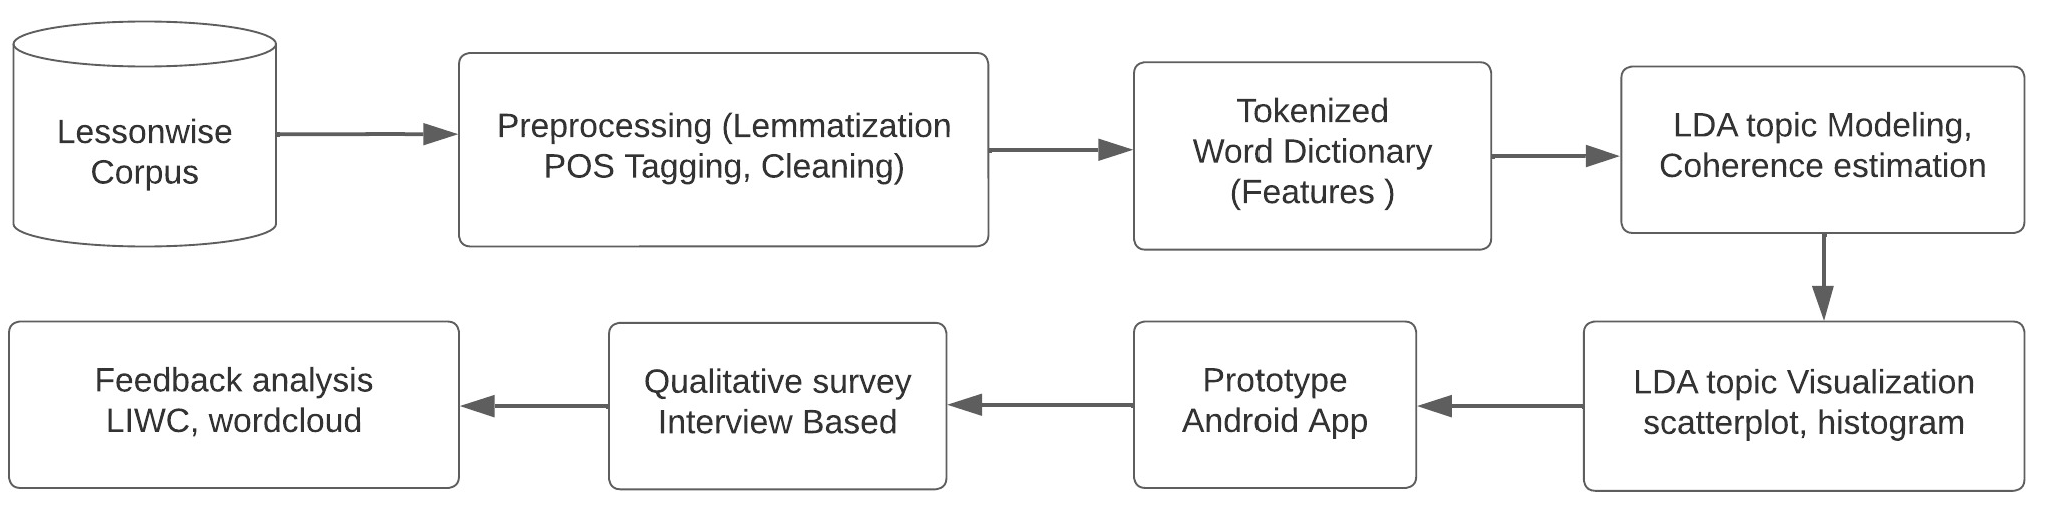
\includegraphics[width=0.9\textwidth]{methodology.png}
\caption{Research workflow diagram}
\end{figure}

LDA algorithm automatically discovers latent topics within the documents based on word co-occurrences. Each topic will be represented by a set of words. Interpret these words to understand the main concepts associated with each topic. Extensive exploratory analysis is conducted to visualize the topic modeling outputs. Analyze the topics generated by the model require manual review and adjustment to ensure the topics make sense.

\subsection{Data Pre-Processing}\label{data_pre}
Text is converted to Lowercased and Normalized to ensure consistent pre-processing \cite{kao_natural_2007}.
  \begin{enumerate}[label=(\roman*)]
  \item
    \textbf{Data cleaning}: unwanted characters, punctuation and special
    character removed and stop words (such as "and," "the," "is," etc)
    are removed. Spacy library's English word model and NLTK's stopwords
    list are used together. Also, words less than two characters are
    removed such as: I, Hi, Oh etc. Hence, Noise is removed and
    irrelevant characters, symbols, or data artifacts that have been
    introduced during data collection or scraping from pdf file to text
    file generation are separated. Hence, we found a cleaned corpus.
  \item
    \textbf{Lemmatization}: Root words are collected words to their dictionary
    form (lemma) is extracted using NLTK's WordNetLemmatizer package.
    Stemming Reduce words to their base or root form is not used since
    sometimes it changes the actual words.
  \item
    \textbf{Part-of-Speech Tagging}: Spacy's English model `en\_core\_web\_sm' is
    used to extract interested words (such as noun, verb, adjective) and
    excluded (CCONJ, AUX, DET, INTJ, PART etc which are Coordinating
    Conjunction, Auxiliary, Determinator, Interjection, Particle etc)
    thereby token is collected for only which are not punctuation,
    conjunction, symbol etc.
  \end{enumerate}

\subsection{Topic Modeling and Feature Extraction}\label{top_mod_feature}
Different techniques have been developed to perform topic modeling in the unsupervised topic modeling domain of Natural Language Processing (NLP), having their own strengths and limitations \cite{vayansky2020review, abdelrazek2022topic, yi2009comparative}. Apart from LDA, Mallet LDA, Structural Topic Model (STM), Hierarchical Dirichlet Process (HDP), Non-Negative Matrix Factorization (NMF), Latent Semantic Analysis (LSA) etc are also prevailing and can be considered for comparative research study. Prevailing LDA based data mining techniques are applied for feature extraction. 

\subsubsection{Latent Dirichlet Allocation (LDA)}
\label{lda_mdel}
LDA model \cite{jelodar_latent_2019, gupta_pan_lda_2021, pichardo_lagunas_svd_lda_2015, selvi_classification_2019} considers documents are mixes of topic, and each topic is a distribution over words. The objective is to derive the hidden topic assignments and the topic-word distributions that most effectively describe the observed documents. The goal of LDA is to uncover these latent topics from a collection of documents without needing any prior labeling or categorization of the content. An expression for the joint distribution of the LDA model is described below:  
\begin{equation}
P(\theta_d,z,w\|\alpha,\beta)=P(\theta_d\|\alpha)\prod^N_{n=1}P(z_{d,n}\|\theta_d)P(w_{d,n}\|z_{d,n},\beta)
\end{equation}
Where $w_{d,n}$ the $n_{th}$ word in document $d$, $z_{d,n}$ the topic assigned to the $n_{th}$ word in document $d$, $\alpha,\beta$ are the Dirichlet LDA model parameters. controls per-document topic distribution, and per topic word distribution. $\theta_d$ represent the topic distribution. $P(\theta_d \| \alpha)$ Dirichlet 
distribution representing the document-topic distribution, $P(z_{d,n}\|\theta_d)$ is the word topic assignment for the $n_{th}$ word in document $d$, $P(w_{d,n}\|z_{d,n},\beta)$ is the distribution representing the observed word given a topic. We have chosen LDA for baseline statistical topic modeling tool. However, how many topics are ideal it is needed to determine and also topic modeling quality needs to measure.

\subsubsection{Comparative analysis of Topic modeling}
While some variations of LDA, Mallet LDA is considered for large corpus processing and analysis \cite{vayansky2020review, abdelrazek2022topic, Comparison_Topic_Modeling_Algorithms}. It focuses on scalability, If large corpus needs to analyze, Mallet LDA might be more suitable. LDA in general can still be efficiently applied to moderately sized corpora. Analyzing topics within the context of metadata, STM could be a better fit. Hierarchical Dirichlet Process (HDP) can be useful when we cannot guess the number of topics in advance. In \cite{Comparison_Topic_Modeling_Algorithms} LSI, NMF and LDA are compared in terms of coherence and similarity measures for social media dataset and in their analysis NMF is observed most effective measures. However, as a baseline model LDA is often considered one of the most prominent choices. In this study Textbook corpus is divided into lessons which is a mixture of topics and using LDA expecting to determine which word in the lesson belong to Lesson\textquotesingle s topics. LDA produces interpretative results for exploratory topic analysis. The identified topics are represented as distributions over words, making it easy to assign meaningful labels to topics. Provided by most of the libraries and tools, making it easy to implement and can be integrated into existing workflows. Hence, LDA serves as a solid baseline for topic modeling tasks.  

\subsubsection{Optimal Topics with Coherence}  
Coherence score measure how coherent or interpret the words in that topic and estimates number of topic clusters \cite{mimno2011optimizing}. Coherence score assess the quality of the topics produced by LDA and ensures that the topics generated are statistically significant. Coherence \(C_{topic}\) can be expressed as follows  
\begin{equation}
C_{topic}=\sum^N_{i=1} \frac{1}{N(N-1)}\sum^i_{j=1} PMI(w_i,w_j)
\end{equation}
Where, \(PMI\left( w_{i},w_{j} \right)\) represent pointwise mutual information statistical association between two words occurring together. PMI score indicates that the two words are more closely related within a topic. \(PMI\left( w_{i},w_{j} \right)\) can expressed as  
\begin{equation}
\(PMI\left( w_{i},w_{j} \right) = \log\frac{P\left( w_{i},w_{j} \right)}{P\left( w_{i} \right)P\left( w_{j} \right)}\)
\end{equation}

where \(P\left( w_{i},w_{j} \right)\) is joint probability of occurrence of words \(w_{i}\) and \(w_{j}\).  To calculate the coherence score gensim library provides range of options such as \(u_{mass},c_{v},c_{uci},c_{npmi}\). \(u_{mass}\) and \(c_{v}\)These two methods are most popular. For given topic with words \(\{ w_{1},w_{2},w_{3},\ldots..,w_{n}\}\) a fixed context window size is provided (default size 10 words) then coherence score is calculated using an equation \(\sum_{j = 1}^{i}{PMI}\left( w_{i},w_{j} \right)\) which provides negative coherence score. \(c_{v}\) can be expressed as  
\begin{equation}
\(c_{v} = \frac{1}{N(N - 1)}\sum_{j = 1}^{i}{similarity\left( w_{i},w_{j} \right)}\)
\end{equation}
in which \(similarity\left( w_{i},w_{j} \right)\) represent the pairwise similarity between terms based on \(PMI\left( w_{i},w_{j} \right)\) scores. \(c_{v}\) provides a positive coherence score. Higher coherence values (higher than 0.5) indicate that the topics are moderately coherent and representative of meaningful themes within the text data.


\subsection{Visualize participants response}\label{vis_part}
\subsubsection{Linguistic Inquiry and Word Count (LIWC)}
\label{liwc}

In this research LIWC is used to ascertain the general sentiment of the
responses given by the survey participants (see section \ref{q_sentiment}). Linguistic Inquiry and Word
Count (LIWC), is a text analysis tool to measure psychological or emotional characteristics \cite{tausczik2010psychological, liwc22_welcome_nodate}. It aims to quantify sentiment by examining the frequencies of different linguistic terms
within given text based on predefined dictionary of words associated
with various categories. Let's assume text as a sequence of words:
\(\left\{ w_{1},w_{2},\ldots.,w_{n} \right\}\) and M different
linguistic categories: \(\left\{ C_{1},C_{2},\ldots.,C_{m} \right\}\) .
Proportion of words in each category
\(P\lbrack i\rbrack = \frac{w\lbrack i\rbrack}{T}\) where T is the total
number of Text. Now, a matrix \(X\lbrack i,j\rbrack\) can be formed,
where \(w_{i}\) represents the frequency of the word in the linguistic
category \(C_{j}\). LIWC vector containing the proportions of words in
each linguistic category can be expressed as
\(P_{total}\lbrack j\rbrack = \frac{\sum_{i = 1}^{T}{X\lbrack i,j\rbrack}}{T}\).

\subsubsection{Word cloud}
\label{wordcloud}
LIWC involves linguistic analysis using mathematical expression but
using word cloud survey answers can be visualized vividly in
interpretable interactive format. Word cloud consider a set of words
\(\left\{ w_{1},w_{2},\ldots.,w_{n} \right\}\) extracted from Text
document and associated frequencies
\(\left\{ f_{1},f_{2},\ldots.,f_{n} \right\}\), \(s_{i}\) represent the
proportional size of the word in the cloud can be expressed as
\(s_{i} = \frac{f_{i}}{\sum_{j = 1}^{n}f_{j}}\) where normalized
frequency \(f_{i}\). In section \ref{q_sentiment} figure \ref{word_cloud_1} and \ref{word_cloud_2} we can see the participants responses most frequent terms. 

\section{Experiment and analysis}\label{exp_analysis}
In this research study for the dataset we have collected Bangladesh NCBI provided English Textbook for class 9-10. Here whole book is segregated into Lessons and we wanted to explore the important topics within the content. Similar topic words remain together. Therefore, assumptions are, it helps students to understands the words, sentences and context of the book. Ideal number of topics are determined using coherence score \cite{mimno2011optimizing}.

\subsection{Coherence measurements}\label{coh_measure}
To measure coherence in the context of LDA, following steps are
followed:

\begin{enumerate}[label=(\roman*)]
\item
  Cleaned document samples are prepared using python's NLP data mining
  techniques explain in detailed in data reprocessing section. Prepared
  \(T\left( d_{i} \right)\) set of tokens in Documents \(d_{i}\) for
  \(i^{th}\) document samples in corpus \(D\).
\item
  Doc to BOW corpus dictionary is prepared with Doc2Bow vector. This
  vector \(x_{d}\) can be represented as where
  \(n\left( w_{i},d \right)\) denotes the count of words \(w_{i}\) for
  the document \(d\).
\item
  Trained LDA Model: During the training phase gensim's MulticoreLDA
  model with four CPU worker thread is set. Doc2Bow dictionary is
  applied along with 20 iterations is invoked. The rest of the
  parameters for LDA model training was default parameter settings of
  gensim library.
\item
  Calculate Coherence: To Calculate the coherence score for each LDA
  model for \(n\) number of topics step 3 is iterated for \(n = 15\)
  times.
\item
  Iteration result coherence score for \(n\) number of topics are saved
  in a list and plotted using seaborn.
\end{enumerate}

\begin{figure}[h!]
\centering
\begin{subfigure}{0.45\textwidth}
    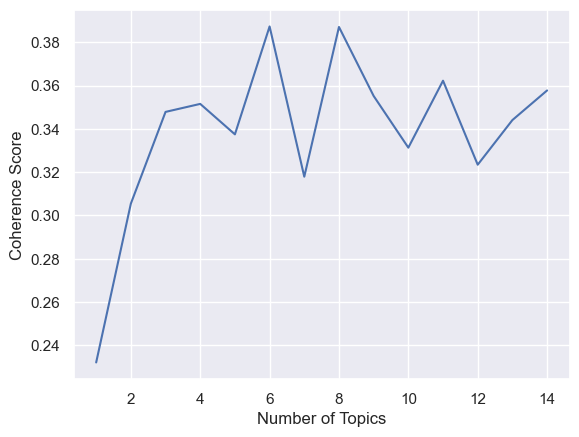
\includegraphics[width=\textwidth]{cv.png}
    \caption{Coherence for $c_v$ approach}
\end{subfigure}
\hfill
\begin{subfigure}{0.45\textwidth}
    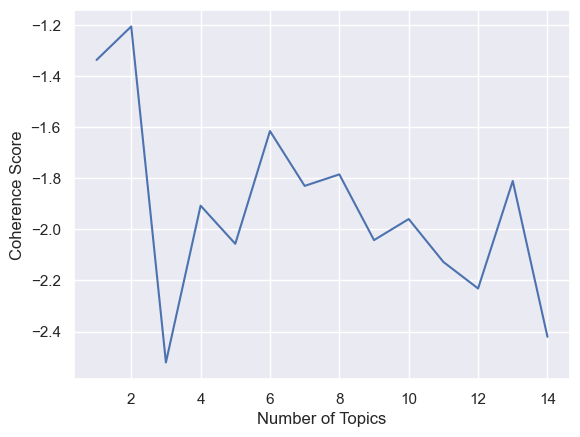
\includegraphics[width=\textwidth]{umass.png}
    \caption{Coherence for $u_{mass}$ approach}
\end{subfigure}       
\caption{Coherence score to estimate optimal number of Topics}
\label{cv_umass}
\end{figure}

From the chart we can see that six topics are dominant in our provided
corpus. The chart shown at the left shows the coherence score for
\(u_{mass}\) and the right chart represents the score for \(c_{v}\) for
multiple iterations. Using 6 topics we can see the output of
corresponding topic and top 10 words in a topic.


\begin{longtable}[]{@{}
  >{\raggedright\arraybackslash}p{(\columnwidth - 4\tabcolsep) * \real{0.17}}     
  >{\raggedright\arraybackslash}p{(\columnwidth - 4\tabcolsep) * \real{0.83}}@{}}
\toprule
Topics & Dominant Keywords and Weights \\
\midrule
\endhead
\textbf{Topic 01} & \enquote*{energy} 0.060, \enquote*{source} 0.029, \enquote*{renewable} 0.018, \enquote*{water}0.016, \enquote*{use} 0.013, \enquote*{gas} 0.013, \enquote*{produce} 0.013, \enquote*{green} 0.013, \enquote*{warm}
0.013, \enquote*{cause} 0.012 
\\
\textbf{Topic 02} & \enquote*{pastime} 0.024, \enquote*{computer} 0.024, \enquote*{social} 0.023, \enquote*{user} 0.022, \enquote*{network} 0.020, \enquote*{student} 0.019, \enquote*{class} 0.017, \enquote*{change} 0.016, \enquote*{book} 0.015, \enquote*{survey} 0.013  
\\
\textbf{Topic 03 }& \enquote*{mother} 0.083, \enquote*{buy} 0.021, \enquote*{love} 0.018, \enquote*{child} 0.014, \enquote*{worker} 0.014, \enquote*{begin} 0.013, \enquote*{cultural} 0.012, \enquote*{observe} 0.012, \enquote*{thing} 0.012, \enquote*{language} 0.011 
\\ 
\textbf{Topic 04} &  \enquote*{life} 0.016, \enquote*{Bangladesh} 0.016, \enquote*{family} 0.015, \enquote*{home} 0.014, \enquote*{root} 0.014, \enquote*{language} 0.014, \enquote*{country} 0.013, \enquote*{Pakistan} 0.010, \enquote*{war} 0.010, \enquote*{man} 0.009 
\\ 
\textbf{Topic 05} & \enquote*{country} 0.031, \enquote*{river} 0.022, \enquote*{India} 0.022, \enquote*{land} 0.021, \enquote*{boat} 0.015, \enquote*{small} 0.015, \enquote*{population} 0.015, \enquote*{lake} 0.013, \enquote*{group} 0.012, \enquote*{house} 0.011 
\\ 
\textbf{Topic 06} & \enquote*{job} 0.064, \enquote*{English} 0.023, \enquote*{learn} 0.021, \enquote*{teacher} 0.017, \enquote*{use} 0.016, \enquote*{dream} 0.016, \enquote*{think} 0.016, \enquote*{thing} 0.015, \enquote*{school} 0.014, \enquote*{education} 0.013\\
\bottomrule
\end{longtable}




%\textbf{Topic 01}: {[}\enquote*{energy} 0.060, \enquote*{source} 0.029, \enquote*{renewable} 0.018, \enquote*{water}
%0.016, \enquote*{use} 0.013, \enquote*{gas} 0.013, \enquote*{produce} 0.013, \enquote*{green} 0.013, \enquote*{warm}
%0.013, \enquote*{cause} 0.012,{]}

%\textbf{Topic 02}: {[}\enquote*{pastime} 0.024, \enquote*{computer} 0.024, \enquote*{social} 0.023, \enquote*{user}
%0.022, \enquote*{network} 0.020, \enquote*{student} 0.019, \enquote*{class} 0.017, \enquote*{change} 0.016,
%\enquote*{book} 0.015, \enquote*{survey} 0.013,{]}

%\textbf{Topic 03}: {[}\enquote*{mother} 0.083, \enquote*{buy} 0.021, \enquote*{love} 0.018, \enquote*{child} 0.014,
%\enquote*{worker} 0.014, \enquote*{begin} 0.013, \enquote*{cultural} 0.012, \enquote*{observe} 0.012,
%\enquote*{thing} 0.012, \enquote*{language} 0.011,{]}

%\textbf{Topic 04}: {[}\enquote*{life} 0.016, \enquote*{Bangladesh} 0.016, \enquote*{family} 0.015, \enquote*{home}
%0.014, \enquote*{root} 0.014, \enquote*{language} 0.014, \enquote*{country} 0.013, \enquote*{Pakistan}
%0.010, \enquote*{war} 0.010, \enquote*{man} 0.009,{]}

%\textbf{Topic 05}: {[}\enquote*{country} 0.031, \enquote*{river} 0.022, \enquote*{India} 0.022, \enquote*{land} 0.021,
%\enquote*{boat} 0.015, \enquote*{small} 0.015, \enquote*{population} 0.015, \enquote*{lake} 0.013, \enquote*{group}
%0.012, \enquote*{house} 0.011,{]}

%\textbf{Topic 06}: {[}\enquote*{job} 0.064, \enquote*{English} 0.023, \enquote*{learn} 0.021, \enquote*{teacher}
%0.017, \enquote*{use} 0.016, \enquote*{dream} 0.016, \enquote*{think} 0.016, \enquote*{thing} 0.015,
%\enquote*{school} 0.014, \enquote*{education} 0.013{]}
\subsection{Dominant topic determination}\label{dom_topic}

In LDA models, each document is composed of multiple topics. But
typically, some specific topics are dominant. The following experiment
extracts this dominant topic for each sentence and shows the relative
weight of the topic and the keywords. It estimated which document
belongs predominantly to which topic. How frequently the words have
appeared in the documents and the weights of each keyword in the same
chart, words that occur in multiple topics and the ones whose relative
frequency is more than the weight.

\subsubsection{Relative Importance measurement}

Word frequency $n(w_{j},d_{i})$ in each document \(D\) is measured in equation \ref{eq:rela_weight} as below which identifies the most frequent words within each document and across the entire corpus.

\begin{equation}
\label{eq:rela_weight}
D = \sum_{d_{i} \in D}^{}\left\{ \begin{array}{l}
1,n\left( w_{i},d_{i} \right) > 0 \\
0,n\left( w_{i},d_{i} \right) = 0 \\
\end{array} \right.\
\end{equation}

we can visualize relative importance of any keywords in terms of frequency and plotted inclined with LDA provided weights (figure \ref{fig:Relative_weight}).

\begin{figure}[h!]
\centering
%\includegraphics[width=18cm, height=10cm,angle=90]{Figs/relative_imp.png}
\includegraphics[width=\textwidth]{relative_imp.png}
\caption{Word frequency and its relative importance}
\label{fig:Relative_weight}
\end{figure}


\subsection{Topic-Term Matrix Visualization}\label{top_term_vis}

Visualizing the topics and their relationships in a topic model Python
library PyLDAvis is used provides an interactive web-based interface to
explore and analyze the LDA results of topic modeling. PyLDAvis itself
abstracts away much of the underlying mathematical complexity and
provides a user-friendly way to generate visualizations and
interactively explore topics and their relationships. Key components
distance among topics and salient terms are explained below:

\subsubsection{Inter-Topic Distance Map}

Distance among topics refers to the measurement of similarity between
topics in a high dimensional space matrix provided by the LDA model.
PyLDAvis library is used to conserve dimensionality reduction using PCA
and for calculating distance between topics metric like Euclidean
distance or Cosine Similarity.

\subsubsection{Salient Terms or dominant keywords}

Salient Terms in a topic are words \(W\) that are most strongly
associated with specific topic. The mathematical expression for finding
salient terms \(w\) for a topic \(t\) involves, extraction of top
\(n\)words that poses the highest probability scores for topic \(t\) in
the topic-term matrix \(P\lbrack t,w\rbrack\).

\begin{figure}[h]
\centerline{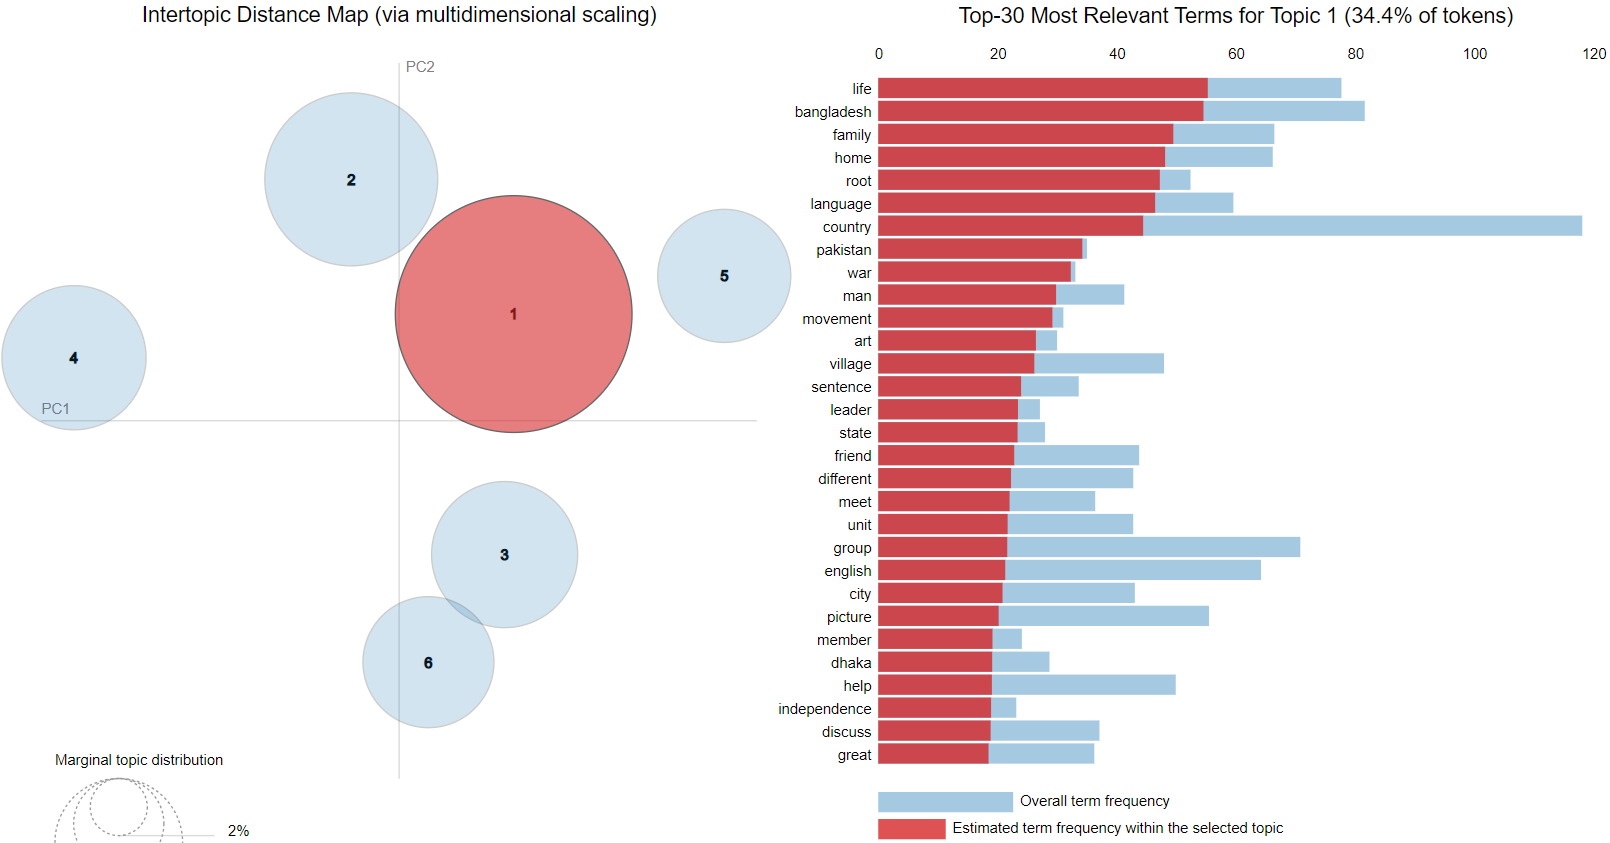
\includegraphics[width=\textwidth]{pyldvis.png}}
\caption{Topic model co-occurrence visualization with dominant keywords'}
\label{Relative_weight_pyldvis}
\end{figure}

Top 30 most salient terms are showed at right in the bar chart histogram
and left figure shows inter topic distance, their size etc (see figure~\ref{Relative_weight_pyldvis}). PCA
dimensionality reduction technique is applied here to embed the LDA
result into a 2D plain scale. Projected the data in lower-dimensional
subspace by computing eigenvalues reduced the circle overlapping. Topics
that are closer together in the map are more similar in terms of the
distribution of words.

\subsection{Qualitative survey}\label{qual_survey}
In the survey questions, it was indicated whether the students, teachers/instructors, and government organizations would find it acceptable and appreciated if textbook information were made available through a mobile app and presented in interactive format. To demonstrate the mobile app idea during the interrogation survey session prototype app Englisher is prepared (see demo in section \ref{Englisher_mobile_app}). Participants were asked for suggestions on how to make the app better and specify shortcomings. Presumably It provides an insight of teacher’s emotion about inclusion of mobile technology in higher secondary English education system. 

\subsubsection{Englisher Mobile App}
\label{Englisher_mobile_app}
A mobile application (Englisher) is being developed with content from the NCTB’s English Textbook for class 9. The extracted keywords are organized into lessons and furthermore quiz is introduced as an exercise. Each sentence's and word's Bengali meaning is provided in accordance with the lesson. Students can take quizzes, and their results are recorded in the history so that history can be reviewed and performance can be improved by more practice in the future. 

\begin{figure}[h!]
\centering
\begin{subfigure}{\textwidth}
	\centering
    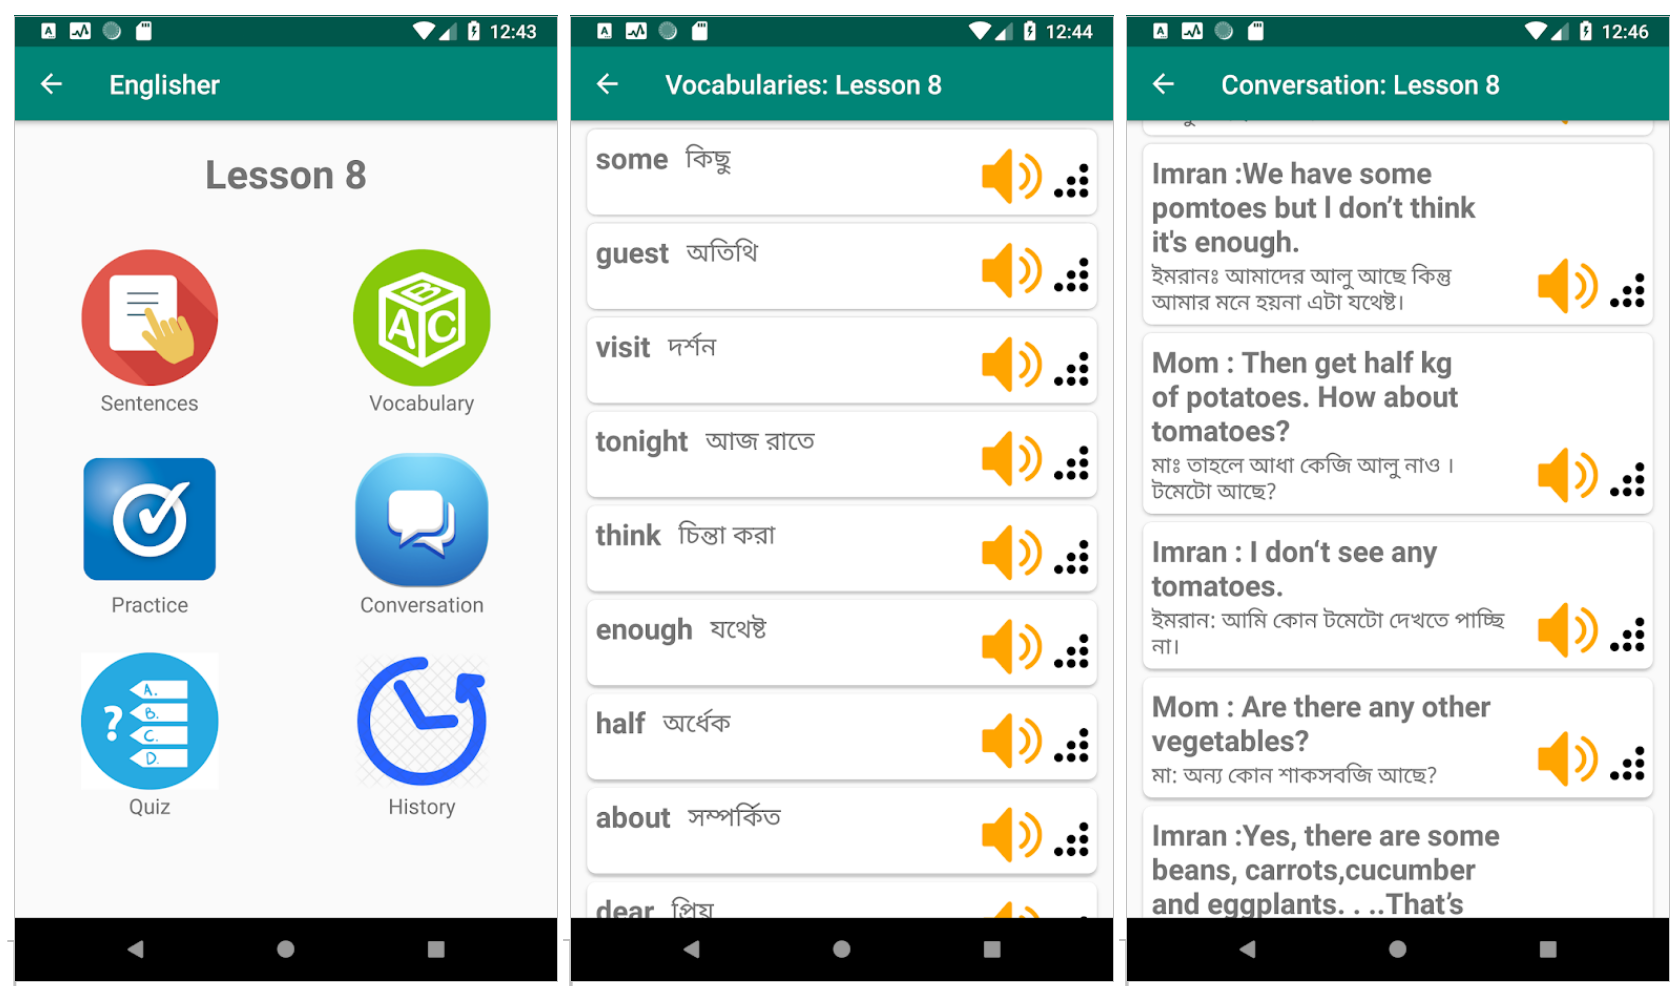
\includegraphics[width=\textwidth]{mobile_app_01.png}
    \caption{Lesson wise exercise}
    \label{fig:first}
\end{subfigure}
\hfill
\begin{subfigure}{\textwidth}
	\centering
    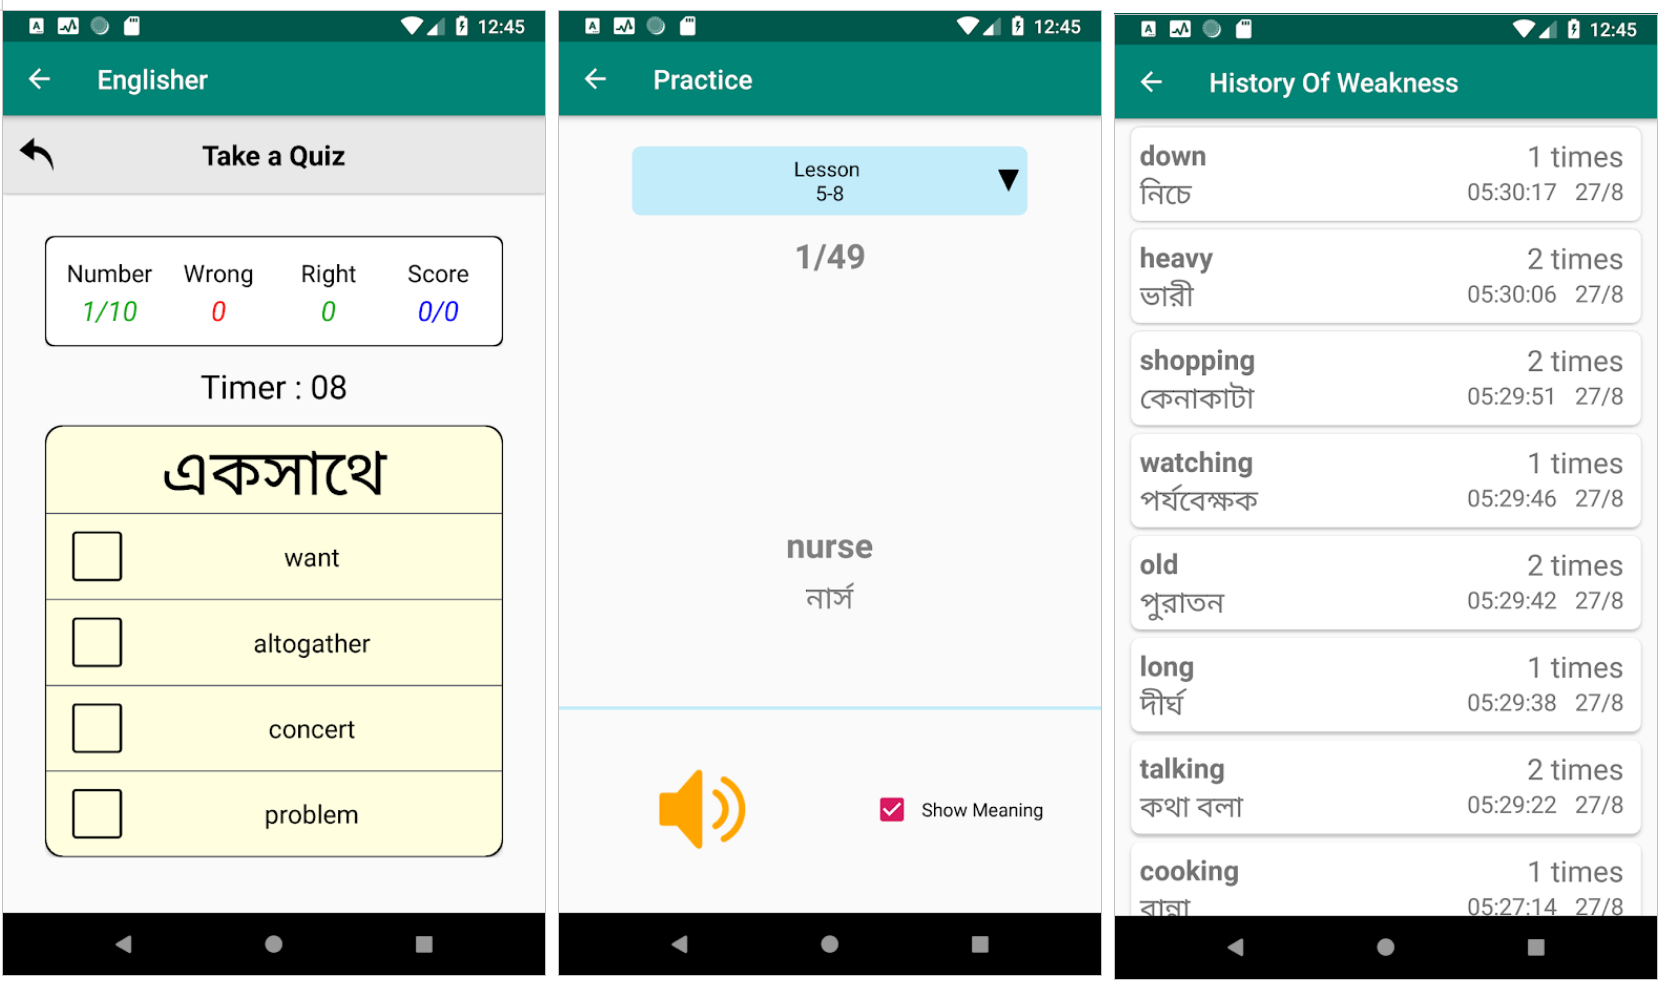
\includegraphics[width=\textwidth]{mobile_app_02.png}
    \caption{Quiz with Vocabulary}
    \label{fig:second}
\end{subfigure}
        
\caption{Englisher Mobile app for Learning LDA based topic model words}
\label{fig:figures}
\end{figure}

\subsubsection{Survey Planning}
The survey was conducted over a period of four weeks, with 50 High schools in Dhaka and Bogura district of Bangladesh. It encompasses only English subject areas Teachers who teaches in high schools from class six to class Ten and teaches regularly in the school. A questionnaire was distributed to teachers allowing us to gather questionnaire answer. 
\subsubsection{Participants}
During the survey standard participants were chosen emphasizing infrastructure quality, teaching experience, class size etc. At the beginning from 100 institution were selected. Then half of them were excluded since those institutions infrastructure's overall quality and condition were not above average. Among the chosen samples 76\% were good and 26\% considered average institutions. Privately held 45\%, 32\% partially government and 22\% are government institutes.  Over 1000 students study in almost 40\% of these institutions and  sizable number of pupils are present in each section and class. 38\% class have a size greater than 50. So, we can presume that the participating teachers have quite a bit of experience teaching sufficient number of students.  
\subsubsection{Survey Results}
We have done extensive analysis with the survey data collected. In our data collection highest priority is given for the secondary class student teachers who teach between 6-10th class about 46\%. High school, KG college and KG High school. Details about the statistics are depicted in the following figure. Adjacent chart explains the percentage of teachers who teach in which class. Hence, from these two figures we can get a vivid image of collected dataset resources about the participating teachers. 

\begin{figure}[h!]
\centering
\begin{subfigure}{0.48\textwidth}
    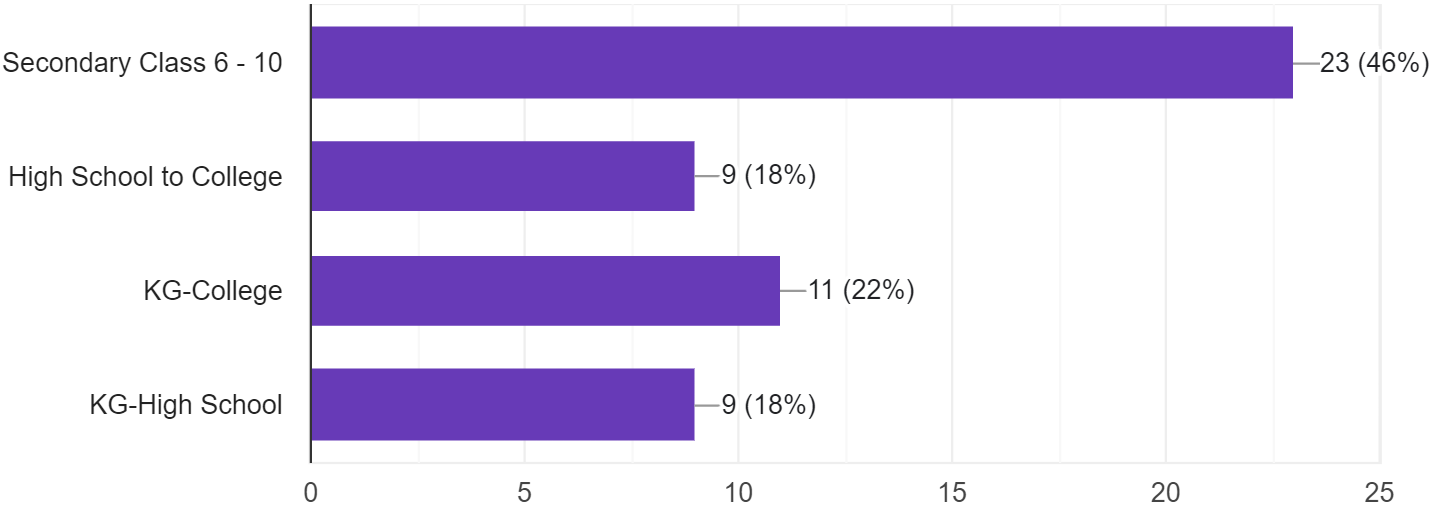
\includegraphics[width=\textwidth]{institution_size.png}
    \caption{Participating institution category and size}
    \label{cv}
\end{subfigure}
\hfill
\begin{subfigure}{0.48\textwidth}
    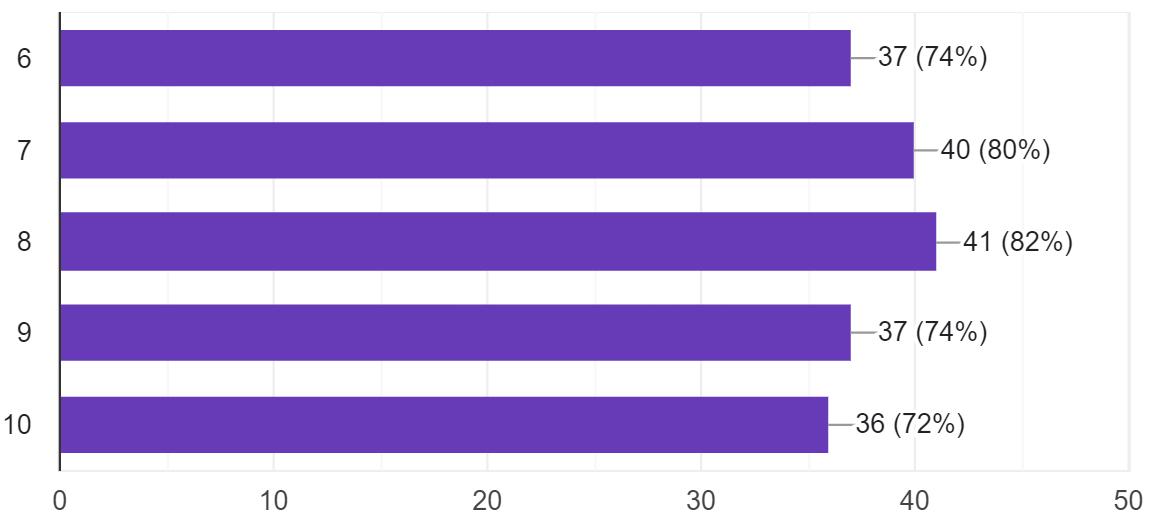
\includegraphics[width=\textwidth]{english_teaching_class.png}
    \caption{Participating instructors' class/Label}
    \label{umass}
\end{subfigure}       
%\caption{Coherence score to estimate optimal number of Topics}
\label{cv_umass}
\end{figure}

The following graphs give an overview of the English teaching experiences of the teachers as well as the general consensus regarding the use of digital content and mobile apps in everyday teaching and learning. Almost 62\% of teachers have been teaching for more than 8 to 10 years, and some of them have been teaching for decades in higher secondary education. 32\% of teachers have three to eight years of experience, while just 6\% are fresh to the profession. Around 83.7\% of teachers the language of instruction during their graduation was English, and their major was also English. Very few teachers 13.3\% graduation major is something other than English yet teaching English in secondary schools probably have sufficient English language proficiency.  

\begin{figure}[h!]
\centering
\begin{subfigure}{0.48\textwidth}
    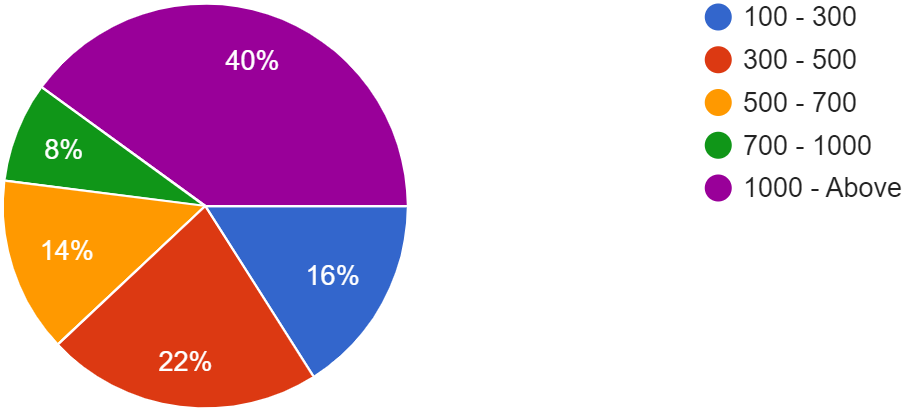
\includegraphics[width=\textwidth]{num_stu.png}
    \caption{Participating institutions' number of students}
    \label{cv}
\end{subfigure}
\hfill
\begin{subfigure}{0.48\textwidth}
    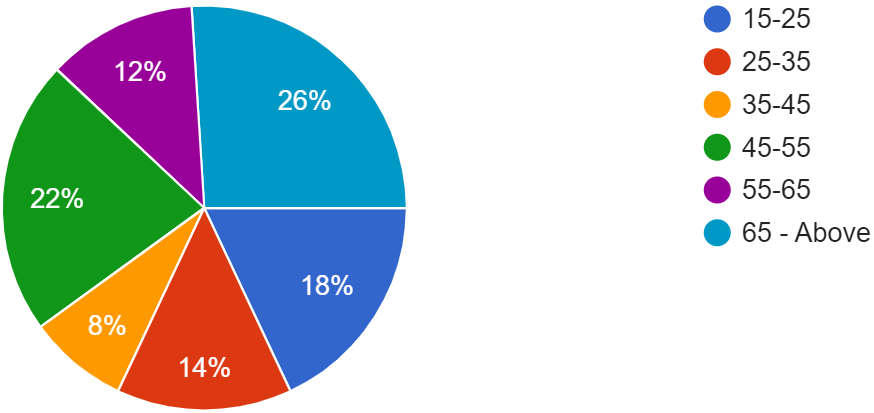
\includegraphics[width=\textwidth]{class_size.png}
    \caption{Participating instructors' class size}
    \label{umass}
\end{subfigure}       
%\caption{Coherence score to estimate optimal number of Topics}
\label{cv_umass}
\end{figure}

\subsubsection{Analyzing survey Facts} 
More than half of teachers, or 58\%, have no prior experience utilizing mobile apps or technology for teaching, but 90\% of them agree, and more than 45\% strongly agree, that it encourages pupils to engage actively in their learning. However, they (almost 60\%) also hold the opinion that a notebook cannot be completely replaced, despite the fact that mobile apps may solve many problems and provide technological support for teaching and learning. Promisingly optimistic approximately 40\%, although thinking that the notebook-based content memorizing learning method can be replaced, feel that mobile app-based learning can replace it permanently. 

\begin{figure}[h!]
\centering
\begin{subfigure}{0.48\textwidth}
    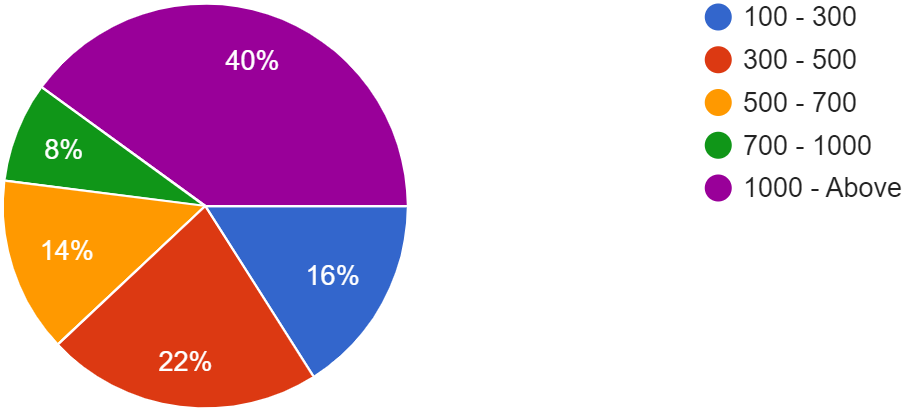
\includegraphics[width=\textwidth]{num_stu.png}
    \caption{Participating institutions' number of students}
    \label{cv}
\end{subfigure}
\hfill
\begin{subfigure}{0.45\textwidth}
    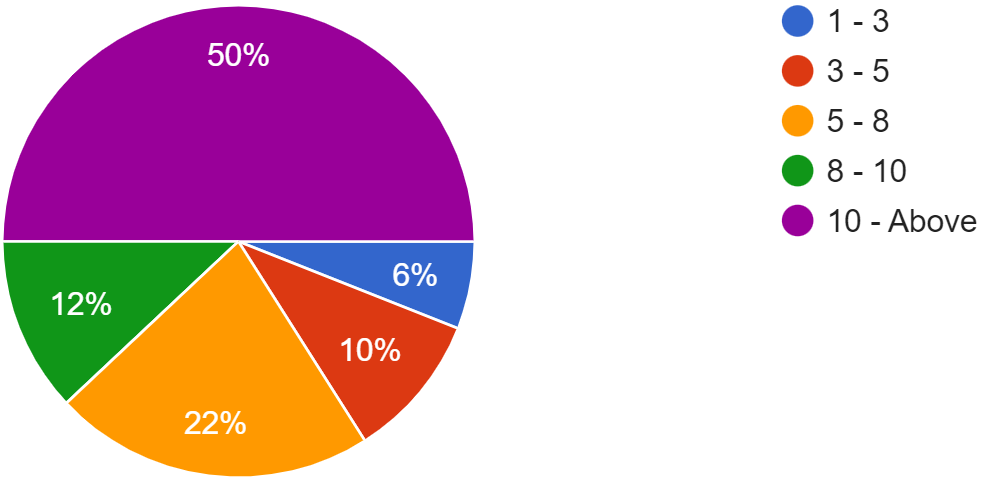
\includegraphics[width=\textwidth]{experience.png}
    \caption{Participating instructors' Teaching experience}
    \label{umass}
\end{subfigure} 
\begin{subfigure}{0.44\textwidth}
    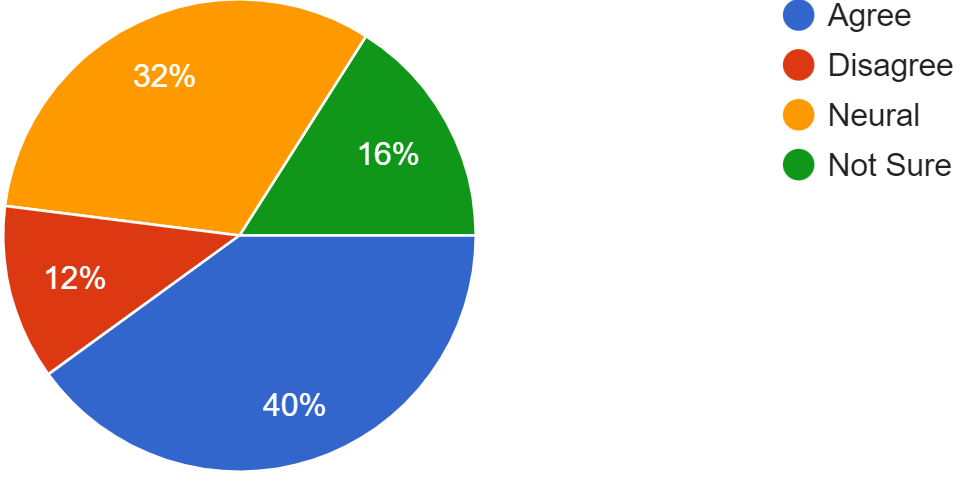
\includegraphics[width=\textwidth]{replace.png}
    \caption{App could help students in replacement of guide book}
    \label{cv}
\end{subfigure}
\hfill
\begin{subfigure}{0.47\textwidth}
    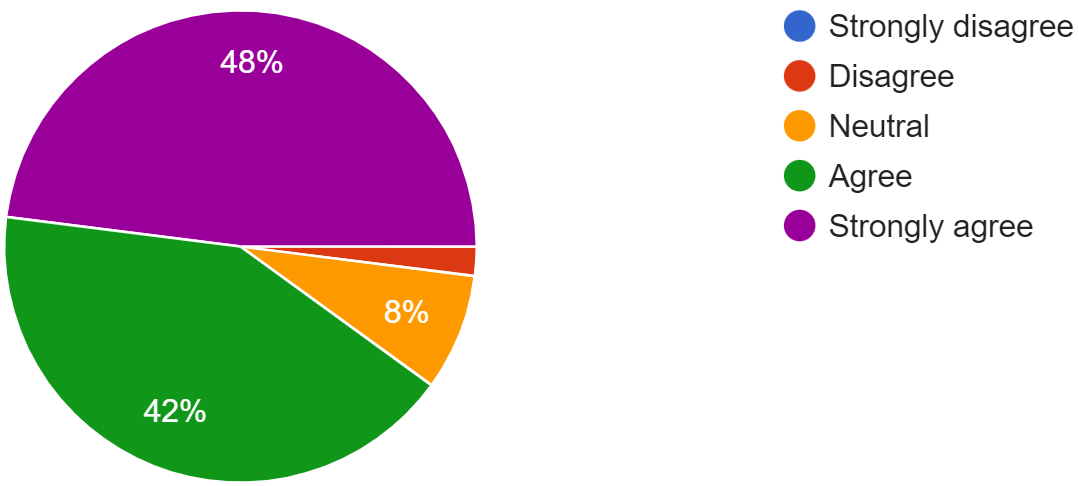
\includegraphics[width=\textwidth]{app_motivates.png}
    \caption{App could motivate students}
    \label{umass}
\end{subfigure}        
%\caption{Coherence score to estimate optimal number of Topics}
\label{cv_umass}
\end{figure}

This study proposes the Englisher mobile app and presents it to the participating teachers to gather their insightful feedback. 92\% of teachers reported that they would use this type of mobile app for teaching if it were made available after using the trial version of the offered customized Englisher app. Teachers anticipate that 80\% of students will utilize this app during class. 86\% of respondents believed it may help students' English proficiency, and 98\% agreed that the government should support this kind of innovation in the education sector. 

\begin{longtable}[]{@{}
  >{\raggedright\arraybackslash}p{(\columnwidth - 4\tabcolsep) * \real{0.7732}}
  >{\raggedright\arraybackslash}p{(\columnwidth - 4\tabcolsep) * \real{0.1066}}
  >{\raggedright\arraybackslash}p{(\columnwidth - 4\tabcolsep) * \real{0.1203}}@{}}
\toprule
\begin{minipage}[b]{\linewidth}\raggedright
\textbf{Questions}
\end{minipage} & \begin{minipage}[b]{\linewidth}\raggedright
\textbf{yes}
\end{minipage} & \begin{minipage}[b]{\linewidth}\raggedright
\textbf{No}
\end{minipage} \\
\midrule
\endhead
Do you use digital content for teaching or digital medium for teaching
and learning? & 84\% & 16\% \\
Have you ever used Internet or Mobile app to teach students or asked
students to find learning materials from internet or Mobile App? & 76\% &
24\% \\
Education during graduation was English and English was used for
learning & 83.70\% & 16.30\% \\
\multicolumn{3}{@{}>{\raggedright\arraybackslash}p{(\columnwidth - 4\tabcolsep) * \real{1.0000} + 4\tabcolsep}@{}}{%
\textit{Customized mobile app for Learning and Teaching English}} \\
Do you think topic model based mobile app-based learning can improve
English proficiency of students? & 86\% & 14\% \\
Do you think Govt should promote these types of innovation for education
sector? & 98\% & 2\% \\
\bottomrule
\end{longtable}

  \subsubsection{Qualitative Survey Sentiment}
  \label{q_sentiment}

\begin{longtable}[]{@{}
  >{\raggedright\arraybackslash}p{(\columnwidth - 12\tabcolsep) * \real{0.1709}}
  >{\raggedright\arraybackslash}p{(\columnwidth - 12\tabcolsep) * \real{0.1042}}
  >{\raggedright\arraybackslash}p{(\columnwidth - 12\tabcolsep) * \real{0.1794}}
  >{\raggedright\arraybackslash}p{(\columnwidth - 12\tabcolsep) * \real{0.1045}}
  >{\raggedright\arraybackslash}p{(\columnwidth - 12\tabcolsep) * \real{0.1756}}
  >{\raggedright\arraybackslash}p{(\columnwidth - 12\tabcolsep) * \real{0.1016}}
  >{\raggedright\arraybackslash}p{(\columnwidth - 12\tabcolsep) * \real{0.1638}}@{}}
\toprule
\begin{minipage}[b]{\linewidth}\raggedright
\textbf{Traditional LIWC Dimension}
\end{minipage} & \begin{minipage}[b]{\linewidth}\raggedright
\textbf{Answer Text}
\end{minipage} & \begin{minipage}[b]{\linewidth}\raggedright
\textbf{Standard Commercial Language}
\end{minipage} & \begin{minipage}[b]{\linewidth}\raggedright
\textbf{Answer Text}
\end{minipage} & \begin{minipage}[b]{\linewidth}\raggedright
\textbf{Standard for Formal Language}
\end{minipage} & \begin{minipage}[b]{\linewidth}\raggedright
\textbf{Answer Text}
\end{minipage} & \begin{minipage}[b]{\linewidth}\raggedright
\textbf{Standard for story language}
\end{minipage} \\
\midrule
\endhead
\textbf{Positive Tone} & 2.54 & 3.96 & 3.91 & 2.33 & 3.22 & 2.18 \\
\textbf{Negative Tone} & 0 & 1.1 & 0 & 1.38 & 0 & 1.75 \\
\textbf{Social Words} & 2.54 & 6.87 & 5.65 & 6.54 & 4.08 & 10.5 \\
\textbf{Cognitive Processes} & 13.56 & 9.35 & 18.26 & 7.95 & 15.88 &
8.7 \\
\textbf{Allure} & 2.54 & 7.79 & 3.04 & 3.58 & 2.79 & 5.48 \\
\textbf{Moralization} & 0 & 0.2 & 0 & 0.3 & 0 & 0.21 \\
\bottomrule
\end{longtable}

From this LIWC table higher proportion of words related to positive
emotions indicate a positive emotional tone in the text in the answer
for the questions related to ``How this app can be improved'' and ``How
English learning can be improved using Mobile App''. LIWC is applied for
three different categories ``commercial writing'', ``Formal language'',
and ``story language'' and in all the categories answer text showed
highly positive sentiment from the survey user. Though respondents had a
mix of optimism and skepticism regarding the use of mobile apps in
teaching and learning. During the interrogation session, their tone was
positive and enticed participants.


\begin{figure}[h!]
\centering
\begin{subfigure}{0.48\textwidth}
    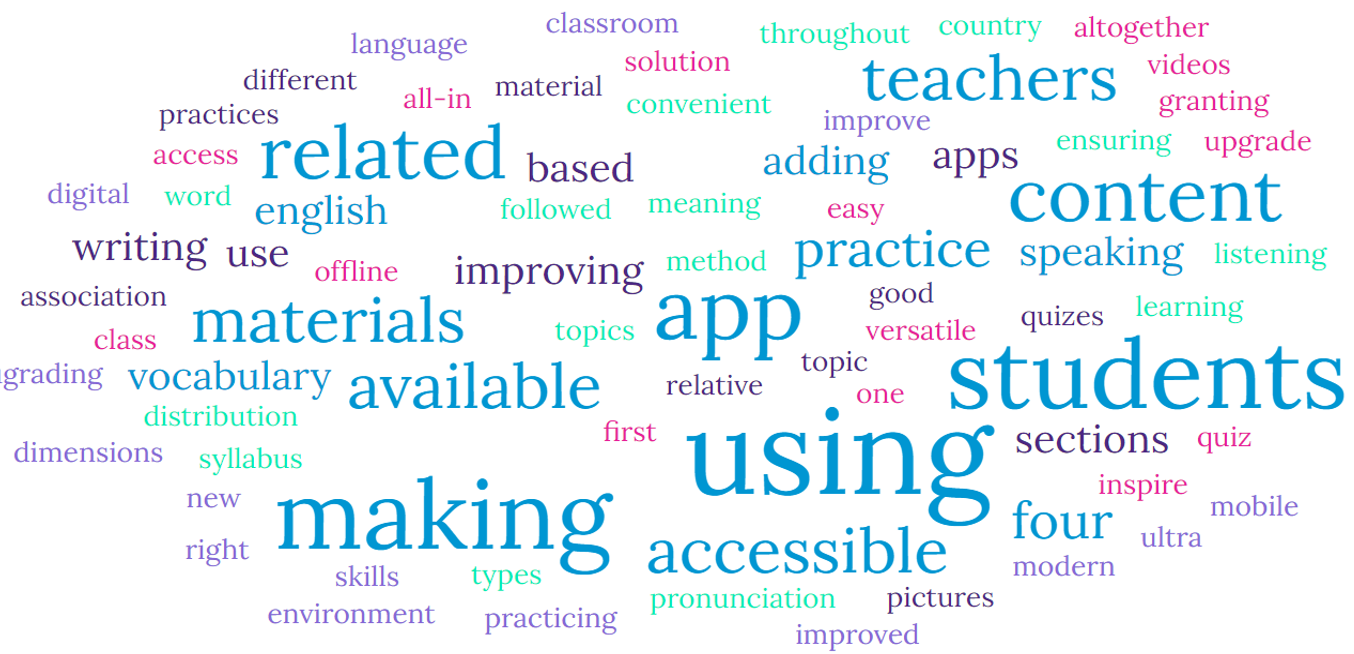
\includegraphics[width=\textwidth]{app_impv.png}
    \caption{word cloud for the question regarding app improvement}
    \label{word_cloud_1}
\end{subfigure}
\hfill
\begin{subfigure}{0.48\textwidth}
    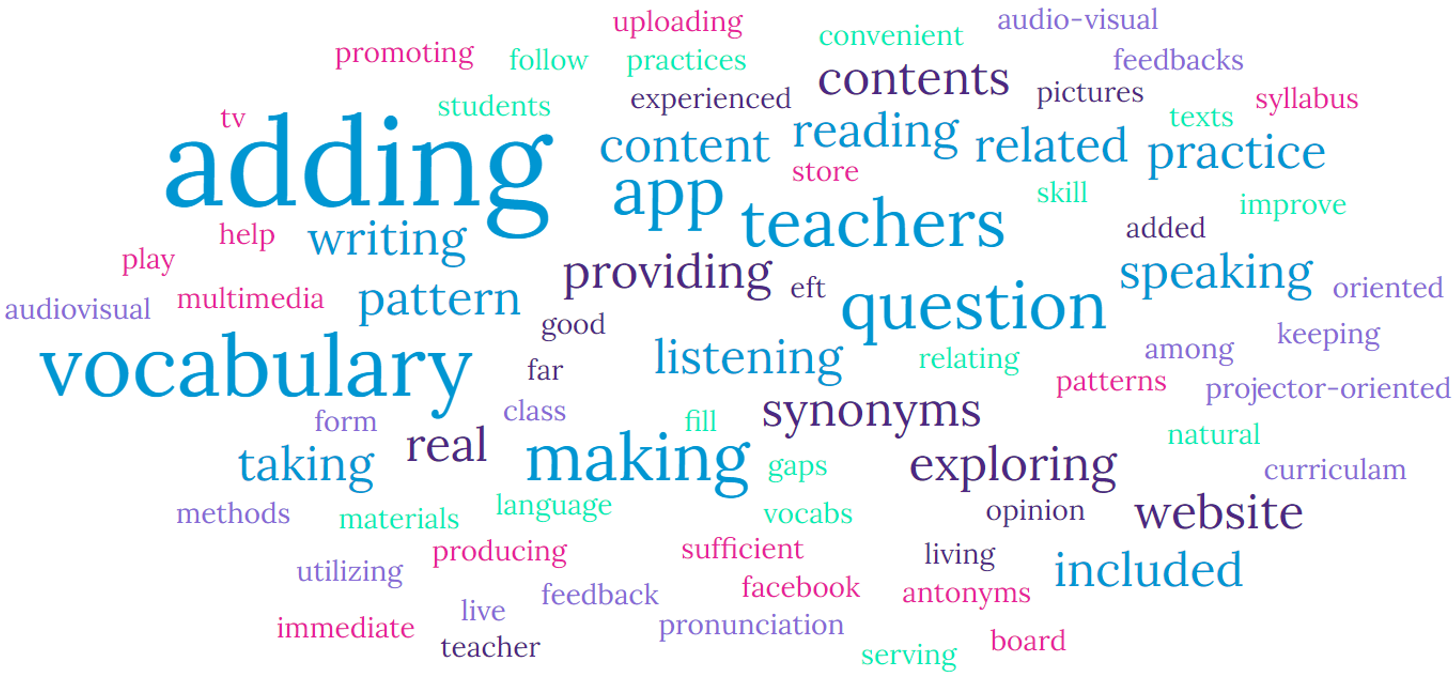
\includegraphics[width=\textwidth]{eng_app_impv.png}
    \caption{word cloud for the question regarding English learning app improvement}
    \label{word_cloud_2}
\end{subfigure}       
%\caption{Coherence score to estimate optimal number of Topics}
\end{figure}

The word cloud is generated from the answers provided question ``how the
app can be improved'' and followed by more generalized question ``how
English learning can be improved using an App''. The participants
narrated varieties of viewpoints for the questions. From the word cloud
it is inferred adding graphical content would enhance the
apps\textquotesingle{} usefulness and make them more visually appealing
to users. More practice resources for listening and exercise would be
helpful. Another suggestion is to include synonym, and syllabus-related
instances as well as audiovisual engagement with the app. Add additional
vocabulary and involve more experience teachers who have greater
experience in digital learning and teaching.

\section{Results Discussion and outcomes}\label{res_dis}

The results demonstrate that LDA-based topic modeling significantly
enhances content comprehension by providing concise summaries of the
learning material. Readers can grasp the main ideas and connections
between topics, aiding in retention and knowledge acquisition. From the
qualitative survey it is revealed LDA based topic modeling approach
based extracted keywords within mobile apps seem effective as it
provides more contextual meaning to the learners. Most of the
participating teachers are enthusiastic about topic modeling based
contexual resources learning related to technology incorporating into
pedagogy. Participants appreciated the cutting edge NLP's learning
resources available through mobile devices. Teachers admitted that
available digital resources facilitated a deeper understanding of topics
and catered to different learning styles, nurturing more engaging
learning environment. This will positively impacted student motivation
and overall engagement and hence boost overall learning. Some crucial
suggestions were improving the graphics of the app so that it becomes
interactive and guardian involvement can be introduced. Based on the
survey results, it is revealed the potential for digital mobile-based
learning in school is immense. Government should take initiatives to
incorporate it into course curriculum syllabus and could impose
ordinance to adopt mobile app based learning teaching in the school.

Apps need to be improved by including collaborative form of learning.
Additionally, the interactive interface receives positive feedback for
its user-friendly design and utility in assisting
readers\textquotesingle{} navigation through the textbook.
Recommendation is to make it specific for NCTB Books only for particular
class. This approach is also our goal considering NCTB Books. Including
interactive e-books, dictionary, educational apps, and multimedia
content.

\section{Limitations}\label{limitat}

LDA could play a role in understanding the topics covered in an English
textbook and potentially aiding in content customization and topic
relevance for personalized learning. In a personalized learning context,
the goal is to tailor the educational experience to the individual needs
and preferences of each learner. This involves understanding the
learner\textquotesingle s strengths, weaknesses, interests, and learning
style. While LDA could be useful in some aspects of this process, it
might not directly address all the requirements of personalized learning
for an English textbook. In this research study we showed that LDA based
topic modeling could be a solution to enhance the context understanding
of the learners. However from the survey it is revealed that app was not
sufficient. Learners oriented topic-document distribution to identify
which topics are most relevant to a specific student can be provided.
App can provide additional explanations, examples, or resources to cater
to their individual learning style. Assessments and exercises focused on
the topics that need reinforcement for each student. Monitor their
progress and adjust the learning path accordingly. Analyze
students\textquotesingle{} performance, engagement, and feedback to
refine the topic modeling process and its integration into the learning
environment. More sophisticated approaches, such as adaptive learning
systems and AI-based tutoring, might be needed to truly personalize the
learning experience in a comprehensive manner.

\section{Special Remarks}

For the data privacy and security issues many Teachers were reluctant to
provide their social website address to the surveyor. Among all the
participants only 24\% attendees provided their social sites address to
use them publicly for research purposes.

\section{Conclusion}\label{conclu}
By employing topic modeling in a personalized learning context,
educators can create more engaging and effective learning experience.
This approach allows enhancement understanding and retention of the
Textbook context. The school survey with prototype app reaffirmed its
potential in learning experiences. LDA based topic modeling leverages
learning experience, improve interpretation and knowledge acquisition.
The synthesis of existing research sheds light on the potential of topic
modeling to improve Textbook context comprehension, and knowledge
retention of learners. It was revealed teachers/instructors would find
it acceptable and appreciated if textbook information were presented
using NLP technology driven algorithms like LDA topic modeling in mobile
app. The study concludes apps seem effective as they provide a personal
and learner-centered learning opportunity ubiquitously. Reveal to user
as a complementary essential material to learn English Textbook quickly
and effectively. The survey\textquotesingle s findings show that teachers are eager to use NLP provided extracted keywords technology in teaching and learning. There are tremendous opportunities, however, apps need to be improved by including
collaborative form of learning.

 

%\section{This is an example for first level head---section head}\label{sec3}
%
%\subsection{This is an example for second level head---subsection head}\label{subsec2}
%
%\subsubsection{This is an example for third level head---subsubsection head}\label{subsubsec2}
%
%Sample body text. Sample body text. Sample body text. Sample body text. Sample body text. Sample body text. Sample body text. Sample body text. 
%
%\section{Equations}\label{sec4}
%
%Equations in \LaTeX\ can either be inline or on-a-line by itself (``display equations''). For
%inline equations use the \verb+$...$+ commands. E.g.: The equation
%$H\psi = E \psi$ is written via the command \verb+$H \psi = E \psi$+.
%
%For display equations (with auto generated equation numbers)
%one can use the equation or align environments:
%\begin{equation}
%\|\tilde{X}(k)\|^2 \leq\frac{\sum\limits_{i=1}^{p}\left\|\tilde{Y}_i(k)\right\|^2+\sum\limits_{j=1}^{q}\left\|\tilde{Z}_j(k)\right\|^2 }{p+q}.\label{eq1}
%\end{equation}
%where,
%\begin{align}
%D_\mu &=  \partial_\mu - ig \frac{\lambda^a}{2} A^a_\mu \nonumber \\
%F^a_{\mu\nu} &= \partial_\mu A^a_\nu - \partial_\nu A^a_\mu + g f^{abc} A^b_\mu A^a_\nu \label{eq2}
%\end{align}
%Notice the use of \verb+\nonumber+ in the align environment at the end
%of each line, except the last, so as not to produce equation numbers on
%lines where no equation numbers are required. The \verb+\label{}+ command
%should only be used at the last line of an align environment where
%\verb+\nonumber+ is not used.
%\begin{equation}
%Y_\infty = \left( \frac{m}{\textrm{GeV}} \right)^{-3}
%    \left[ 1 + \frac{3 \ln(m/\textrm{GeV})}{15}
%    + \frac{\ln(c_2/5)}{15} \right]
%\end{equation}
%The class file also supports the use of \verb+\mathbb{}+, \verb+\mathscr{}+ and
%\verb+\mathcal{}+ commands. As such \verb+\mathbb{R}+, \verb+\mathscr{R}+
%and \verb+\mathcal{R}+ produces $\mathbb{R}$, $\mathscr{R}$ and $\mathcal{R}$
%respectively (refer Subsubsection~\ref{subsubsec2}).
%
%\section{Tables}\label{sec5}
%
%Tables can be inserted via the normal table and tabular environment. To put
%footnotes inside tables you should use \verb+\footnotetext[]{...}+ tag.
%The footnote appears just below the table itself (refer Tables~\ref{tab1} and \ref{tab2}). 
%For the corresponding footnotemark use \verb+\footnotemark[...]+
%


\noindent



%%=============================================%%
%% For presentation purpose, we have included  %%
%% \bigskip command. please ignore this.       %%
%%=============================================%%

%%=============================================%%
%%% For presentation purpose, we have included  %%
%%% \bigskip command. please ignore this.       %%
%%%=============================================%%
%
%\begin{table}[h]
%\begin{center}
%\begin{minipage}{\textwidth}
%\caption{Example of a lengthy table which is set to full textwidth}\label{tab2}
%\begin{tabular*}{\textwidth}{@{\extracolsep{\fill}}lcccccc@{\extracolsep{\fill}}}
%\toprule%
%& \multicolumn{3}{@{}c@{}}{Element 1\footnotemark[1]} & \multicolumn{3}{@{}c@{}}{Element 2\footnotemark[2]} \\\cmidrule{2-4}\cmidrule{5-7}%
%Project & Energy & $\sigma_{calc}$ & $\sigma_{expt}$ & Energy & $\sigma_{calc}$ & $\sigma_{expt}$ \\
%\midrule
%Element 3  & 990 A & 1168 & $1547\pm12$ & 780 A & 1166 & $1239\pm100$\\
%Element 4  & 500 A & 961  & $922\pm10$  & 900 A & 1268 & $1092\pm40$\\
%\botrule
%\end{tabular*}
%\footnotetext{Note: This is an example of table footnote. This is an example of table footnote this is an example of table footnote this is an example of~table footnote this is an example of table footnote.}
%\footnotetext[1]{Example for a first table footnote.}
%\footnotetext[2]{Example for a second table footnote.}
%\end{minipage}
%\end{center}
%\end{table}
%
%In case of double column layout, tables which do not fit in single column width should be set to full text width. For this, you need to use \verb+\begin{table*}+ \verb+...+ \verb+\end{table*}+ instead of \verb+\begin{table}+ \verb+...+ \verb+\end{table}+ environment. Lengthy tables which do not fit in textwidth should be set as rotated table. For this, you need to use \verb+\begin{sidewaystable}+ \verb+...+ \verb+\end{sidewaystable}+ instead of \verb+\begin{table*}+ \verb+...+ \verb+\end{table*}+ environment. This environment puts tables rotated to single column width. For tables rotated to double column width, use \verb+\begin{sidewaystable*}+ \verb+...+ \verb+\end{sidewaystable*}+.
%
%\begin{sidewaystable}
%\sidewaystablefn%
%\begin{center}
%\begin{minipage}{\textheight}
%\caption{Tables which are too long to fit, should be written using the ``sidewaystable'' environment as shown here}\label{tab3}
%\begin{tabular*}{\textheight}{@{\extracolsep{\fill}}lcccccc@{\extracolsep{\fill}}}
%\toprule%
%& \multicolumn{3}{@{}c@{}}{Element 1\footnotemark[1]}& \multicolumn{3}{@{}c@{}}{Element\footnotemark[2]} \\\cmidrule{2-4}\cmidrule{5-7}%
%Projectile & Energy	& $\sigma_{calc}$ & $\sigma_{expt}$ & Energy & $\sigma_{calc}$ & $\sigma_{expt}$ \\
%\midrule
%Element 3 & 990 A & 1168 & $1547\pm12$ & 780 A & 1166 & $1239\pm100$ \\
%Element 4 & 500 A & 961  & $922\pm10$  & 900 A & 1268 & $1092\pm40$ \\
%Element 5 & 990 A & 1168 & $1547\pm12$ & 780 A & 1166 & $1239\pm100$ \\
%Element 6 & 500 A & 961  & $922\pm10$  & 900 A & 1268 & $1092\pm40$ \\
%\botrule
%\end{tabular*}
%\footnotetext{Note: This is an example of table footnote this is an example of table footnote this is an example of table footnote this is an example of~table footnote this is an example of table footnote.}
%\footnotetext[1]{This is an example of table footnote.}
%\end{minipage}
%\end{center}
%\end{sidewaystable}
%
%\section{Figures}\label{sec6}
%
%As per the \LaTeX\ standards you need to use eps images for \LaTeX\ compilation and \verb+pdf/jpg/png+ images for \verb+PDFLaTeX+ compilation. This is one of the major difference between \LaTeX\ and \verb+PDFLaTeX+. Each image should be from a single input .eps/vector image file. Avoid using subfigures. The command for inserting images for \LaTeX\ and \verb+PDFLaTeX+ can be generalized. The package used to insert images in \verb+LaTeX/PDFLaTeX+ is the graphicx package. Figures can be inserted via the normal figure environment as shown in the below example:
%
%%%=============================================%%
%%% For presentation purpose, we have included  %%
%%% \bigskip command. please ignore this.       %%
%%%=============================================%%
%\bigskip
%\begin{verbatim}
%\begin{figure}[<placement-specifier>]
%\centering
%\includegraphics{<eps-file>}
%\caption{<figure-caption>}\label{<figure-label>}
%\end{figure}
%\end{verbatim}
%\bigskip
%%%=============================================%%
%%% For presentation purpose, we have included  %%
%%% \bigskip command. please ignore this.       %%
%%%=============================================%%
%
%\begin{figure}[h]%
%\centering
%
\includegraphics[width=0.9\textwidth]{fig.eps}
%\caption{This is a widefig. This is an example of long caption this is an example of long caption  this is an example of long caption this is an example of long caption}\label{fig1}
%\end{figure}
%
%In case of double column layout, the above format puts figure captions/images to single column width. To get spanned images, we need to provide \verb+\begin{figure*}+ \verb+...+ \verb+\end{figure*}+.
%
%For sample purpose, we have included the width of images in the optional argument of \verb+\includegraphics+ tag. Please ignore this. 
%
%\section{Algorithms, Program codes and Listings}\label{sec7}
%
%Packages \verb+algorithm+, \verb+algorithmicx+ and \verb+algpseudocode+ are used for setting algorithms in \LaTeX\ using the format:
%
%%%=============================================%%
%%% For presentation purpose, we have included  %%
%%% \bigskip command. please ignore this.       %%
%%%=============================================%%
%\bigskip
%\begin{verbatim}
%\begin{algorithm}
%\caption{<alg-caption>}\label{<alg-label>}
%\begin{algorithmic}[1]
%. . .
%\end{algorithmic}
%\end{algorithm}
%\end{verbatim}
%\bigskip
%%%=============================================%%
%%% For presentation purpose, we have included  %%
%%% \bigskip command. please ignore this.       %%
%%%=============================================%%
%
%You may refer above listed package documentations for more details before setting \verb+algorithm+ environment. For program codes, the ``program'' package is required and the command to be used is \verb+\begin{program}+ \verb+...+ \verb+\end{program}+. A fast exponentiation procedure:
%
%\begin{program}
%\BEGIN \\ %
%  \FOR i:=1 \TO 10 \STEP 1 \DO
%     |expt|(2,i); \\ |newline|() \OD %
%\rcomment{Comments will be set flush to the right margin}
%\WHERE
%\PROC |expt|(x,n) \BODY
%          z:=1;
%          \DO \IF n=0 \THEN \EXIT \FI;
%             \DO \IF |odd|(n) \THEN \EXIT \FI;
%\COMMENT{This is a comment statement};
%                n:=n/2; x:=x*x \OD;
%             \{ n>0 \};
%             n:=n-1; z:=z*x \OD;
%          |print|(z) \ENDPROC
%\END
%\end{program}
%
%
%\begin{algorithm}
%\caption{Calculate $y = x^n$}\label{algo1}
%\begin{algorithmic}[1]
%\Require $n \geq 0 \vee x \neq 0$
%\Ensure $y = x^n$ 
%\State $y \Leftarrow 1$
%\If{$n < 0$}\label{algln2}
%        \State $X \Leftarrow 1 / x$
%        \State $N \Leftarrow -n$
%\Else
%        \State $X \Leftarrow x$
%        \State $N \Leftarrow n$
%\EndIf
%\While{$N \neq 0$}
%        \If{$N$ is even}
%            \State $X \Leftarrow X \times X$
%            \State $N \Leftarrow N / 2$
%        \Else[$N$ is odd]
%            \State $y \Leftarrow y \times X$
%            \State $N \Leftarrow N - 1$
%        \EndIf
%\EndWhile
%\end{algorithmic}
%\end{algorithm}
%\bigskip
%%%=============================================%%
%%% For presentation purpose, we have included  %%
%%% \bigskip command. please ignore this.       %%
%%%=============================================%%
%
%Similarly, for \verb+listings+, use the \verb+listings+ package. \verb+\begin{lstlisting}+ \verb+...+ \verb+\end{lstlisting}+ is used to set environments similar to \verb+verbatim+ environment. Refer to the \verb+lstlisting+ package documentation for more details.
%
%%%=============================================%%
%%% For presentation purpose, we have included  %%
%%% \bigskip command. please ignore this.       %%
%%%=============================================%%
%\bigskip
%\begin{minipage}{\hsize}%
%\lstset{frame=single,framexleftmargin=-1pt,framexrightmargin=-17pt,framesep=12pt,linewidth=0.98\textwidth,language=pascal}% Set your language (you can change the language for each code-block optionally)
%%%% Start your code-block
%\begin{lstlisting}
%for i:=maxint to 0 do
%begin
%{ do nothing }
%end;
%Write('Case insensitive ');
%Write('Pascal keywords.');
%\end{lstlisting}
%\end{minipage}
%
%\section{Cross referencing}\label{sec8}
%
%Environments such as figure, table, equation and align can have a label
%declared via the \verb+\label{#label}+ command. For figures and table
%environments use the \verb+\label{}+ command inside or just
%below the \verb+\caption{}+ command. You can then use the
%\verb+\ref{#label}+ command to cross-reference them. As an example, consider
%the label declared for Figure~\ref{fig1} which is
%\verb+\label{fig1}+. To cross-reference it, use the command 
%\verb+Figure \ref{fig1}+, for which it comes up as
%``Figure~\ref{fig1}''. 
%
%To reference line numbers in an algorithm, consider the label declared for the line number 2 of Algorithm~\ref{algo1} is \verb+\label{algln2}+. To cross-reference it, use the command \verb+\ref{algln2}+ for which it comes up as line~\ref{algln2} of Algorithm~\ref{algo1}.
%
%\subsection{Details on reference citations}\label{subsec7}
%
%Standard \LaTeX\ permits only numerical citations. To support both numerical and author-year citations this template uses \verb+natbib+ \LaTeX\ package. For style guidance please refer to the template user manual.
%
%Here is an example for \verb+\cite{...}+: \cite{bib1}. Another example for \verb+\citep{...}+: \citep{bib2}. For author-year citation mode, \verb+\cite{...}+ prints Jones et al. (1990) and \verb+\citep{...}+ prints (Jones et al., 1990).
%
%All cited bib entries are printed at the end of this article: \cite{bib3}, \cite{bib4}, \cite{bib5}, \cite{bib6}, \cite{bib7}, \cite{bib8}, \cite{bib9}, \cite{bib10}, \cite{bib11} and \cite{bib12}.
%
%\section{Examples for theorem like environments}\label{sec10}
%
%For theorem like environments, we require \verb+amsthm+ package. There are three types of predefined theorem styles exists---\verb+thmstyleone+, \verb+thmstyletwo+ and \verb+thmstylethree+ 
%
%%%=============================================%%
%%% For presentation purpose, we have included  %%
%%% \bigskip command. please ignore this.       %%
%%%=============================================%%
%\bigskip
%\begin{tabular}{|l|p{19pc}|}
%\hline
%\verb+thmstyleone+ & Numbered, theorem head in bold font and theorem text in italic style \\\hline
%\verb+thmstyletwo+ & Numbered, theorem head in roman font and theorem text in italic style \\\hline
%\verb+thmstylethree+ & Numbered, theorem head in bold font and theorem text in roman style \\\hline
%\end{tabular}
%\bigskip
%%%=============================================%%
%%% For presentation purpose, we have included  %%
%%% \bigskip command. please ignore this.       %%
%%%=============================================%%
%
%For mathematics journals, theorem styles can be included as shown in the following examples:
%
%\begin{theorem}[Theorem subhead]\label{thm1}
%Example theorem text. Example theorem text. Example theorem text. Example theorem text. Example theorem text. 
%Example theorem text. Example theorem text. Example theorem text. Example theorem text. Example theorem text. 
%Example theorem text. 
%\end{theorem}
%
%Sample body text. Sample body text. Sample body text. Sample body text. Sample body text. Sample body text. Sample body text. Sample body text.
%
%\begin{proposition}
%Example proposition text. Example proposition text. Example proposition text. Example proposition text. Example proposition text. 
%Example proposition text. Example proposition text. Example proposition text. Example proposition text. Example proposition text. 
%\end{proposition}
%
%Sample body text. Sample body text. Sample body text. Sample body text. Sample body text. Sample body text. Sample body text. Sample body text.
%
%\begin{example}
%Phasellus adipiscing semper elit. Proin fermentum massa
%ac quam. Sed diam turpis, molestie vitae, placerat a, molestie nec, leo. Maecenas lacinia. Nam ipsum ligula, eleifend
%at, accumsan nec, suscipit a, ipsum. Morbi blandit ligula feugiat magna. Nunc eleifend consequat lorem. 
%\end{example}
%
%Sample body text. Sample body text. Sample body text. Sample body text. Sample body text. Sample body text. Sample body text. Sample body text.
%
%\begin{remark}
%Phasellus adipiscing semper elit. Proin fermentum massa
%ac quam. Sed diam turpis, molestie vitae, placerat a, molestie nec, leo. Maecenas lacinia. Nam ipsum ligula, eleifend
%at, accumsan nec, suscipit a, ipsum. Morbi blandit ligula feugiat magna. Nunc eleifend consequat lorem. 
%\end{remark}
%
%Sample body text. Sample body text. Sample body text. Sample body text. Sample body text. Sample body text. Sample body text. Sample body text.
%
%\begin{definition}[Definition sub head]
%Example definition text. Example definition text. Example definition text. Example definition text. Example definition text. Example definition text. Example definition text. Example definition text. 
%\end{definition}
%
%Additionally a predefined ``proof'' environment is available: \verb+\begin{proof}+ \verb+...+ \verb+\end{proof}+. This prints a ``Proof'' head in italic font style and the ``body text'' in roman font style with an open square at the end of each proof environment. 
%
%\begin{proof}
%Example for proof text. Example for proof text. Example for proof text. Example for proof text. Example for proof text. Example for proof text. Example for proof text. Example for proof text. Example for proof text. Example for proof text. 
%\end{proof}
%
%Sample body text. Sample body text. Sample body text. Sample body text. Sample body text. Sample body text. Sample body text. Sample body text.
%
%\begin{proof}[Proof of Theorem~{\upshape\ref{thm1}}]
%Example for proof text. Example for proof text. Example for proof text. Example for proof text. Example for proof text. Example for proof text. Example for proof text. Example for proof text. Example for proof text. Example for proof text. 
%\end{proof}
%
%\noindent
%For a quote environment, use \verb+\begin{quote}...\end{quote}+
%\begin{quote}
%Quoted text example. Aliquam porttitor quam a lacus. Praesent vel arcu ut tortor cursus volutpat. In vitae pede quis diam bibendum placerat. Fusce elementum
%convallis neque. Sed dolor orci, scelerisque ac, dapibus nec, ultricies ut, mi. Duis nec dui quis leo sagittis commodo.
%\end{quote}
%
%Sample body text. Sample body text. Sample body text. Sample body text. Sample body text (refer Figure~\ref{fig1}). Sample body text. Sample body text. Sample body text (refer Table~\ref{tab3}). 
%
%\section{Methods}\label{sec11}
%
%Topical subheadings are allowed. Authors must ensure that their Methods section includes adequate experimental and characterization data necessary for others in the field to reproduce their work. Authors are encouraged to include RIIDs where appropriate. 
%
%\textbf{Ethical approval declarations} (only required where applicable) Any article reporting experiment/s carried out on (i)~live vertebrate (or higher invertebrates), (ii)~humans or (iii)~human samples must include an unambiguous statement within the methods section that meets the following requirements: 
%
%\begin{enumerate}[1.]
%\item Approval: a statement which confirms that all experimental protocols were approved by a named institutional and/or licensing committee. Please identify the approving body in the methods section
%
%\item Accordance: a statement explicitly saying that the methods were carried out in accordance with the relevant guidelines and regulations
%
%\item Informed consent (for experiments involving humans or human tissue samples): include a statement confirming that informed consent was obtained from all participants and/or their legal guardian/s
%\end{enumerate}
%
%If your manuscript includes potentially identifying patient/participant information, or if it describes human transplantation research, or if it reports results of a clinical trial then  additional information will be required. Please visit (\url{https://www.nature.com/nature-research/editorial-policies}) for Nature Portfolio journals, (\url{https://www.springer.com/gp/authors-editors/journal-author/journal-author-helpdesk/publishing-ethics/14214}) for Springer Nature journals, or (\url{https://www.biomedcentral.com/getpublished/editorial-policies\#ethics+and+consent}) for BMC.
%
%\section{Discussion}\label{sec12}
%
%Discussions should be brief and focused. In some disciplines use of Discussion or `Conclusion' is interchangeable. It is not mandatory to use both. Some journals prefer a section `Results and Discussion' followed by a section `Conclusion'. Please refer to Journal-level guidance for any specific requirements. 
%
%\section{Conclusion}\label{sec13}
%
%From the analysis we found there are strong correlation within the features among this two categories depression and suicide post. The most frequent words of two categories has similarities. After using the exploratory analysis using scatterplot we saw many words which seems to be a written post word from depressed person appears within suicide category. During analysis one interesting result is observed that depression persons post is relatively shorter and full of abusive words. Simple Term frequency based vectorization technique could not effectively estimates the depression impact. Surprisingly, after analysis with TFIDF and countvectorization methods we found that there is 99\% chance that the person who is depressed also has suicial tendency. Here, gridsearch technique is used to determine the best classification estimator. Since, vectorizer is not trained with the reddit dataset. Hence, we are assuming that after getting the result the vectors are not god enough to classify right way. Also, another reason is we compelled the classifier to classify the samples in suicidal risk categories. Hence, it does not have a choice rather than label the sample to suicidal risk category.  
%
%\backmatter
%
%\bmhead{Supplementary information}
%
%If your article has accompanying supplementary file/s please state so here. 
%
%Authors reporting data from electrophoretic gels and blots should supply the full unprocessed scans for key as part of their Supplementary information. This may be requested by the editorial team/s if it is missing.
%
%Please refer to Journal-level guidance for any specific requirements.
%
%\bmhead{Acknowledgments}
%
%Acknowledgments are not compulsory. Where included they should be brief. Grant or contribution numbers may be acknowledged.
%
%Please refer to Journal-level guidance for any specific requirements.
%
%\section*{Declarations}
%
%Some journals require declarations to be submitted in a standardised format. Please check the Instructions for Authors of the journal to which you are submitting to see if you need to complete this section. If yes, your manuscript must contain the following sections under the heading `Declarations':
%
%\begin{itemize}
%\item Funding
%\item Conflict of interest/Competing interests (check journal-specific guidelines for which heading to use)
%\item Ethics approval 
%\item Consent to participate
%\item Consent for publication
%\item Availability of data and materials
%\item Code availability 
%\item Authors' contributions
%\end{itemize}
%
%\noindent
%If any of the sections are not relevant to your manuscript, please include the heading and write `Not applicable' for that section. 
%
%%%===================================================%%
%%% For presentation purpose, we have included        %%
%%% \bigskip command. please ignore this.             %%
%%%===================================================%%
%\bigskip
%\begin{flushleft}%
%Editorial Policies for:
%
%\bigskip\noindent
%Springer journals and proceedings: \url{https://www.springer.com/gp/editorial-policies}
%
%\bigskip\noindent
%Nature Portfolio journals: \url{https://www.nature.com/nature-research/editorial-policies}
%
%\bigskip\noindent
%\textit{Scientific Reports}: \url{https://www.nature.com/srep/journal-policies/editorial-policies}
%
%\bigskip\noindent
%BMC journals: \url{https://www.biomedcentral.com/getpublished/editorial-policies}
%\end{flushleft}
%
%\begin{appendices}
%
%\section{Section title of first appendix}\label{secA1}
%
%An appendix contains supplementary information that is not an essential part of the text itself but which may be helpful in providing a more comprehensive understanding of the research problem or it is information that is too cumbersome to be included in the body of the paper.
%
%%%=============================================%%
%%% For submissions to Nature Portfolio Journals %%
%%% please use the heading ``Extended Data''.   %%
%%%=============================================%%
%
%%%=============================================================%%
%%% Sample for another appendix section			       %%
%%%=============================================================%%
%
%%% \section{Example of another appendix section}\label{secA2}%
%%% Appendices may be used for helpful, supporting or essential material that would otherwise 
%%% clutter, break up or be distracting to the text. Appendices can consist of sections, figures, 
%%% tables and equations etc.
%
%\end{appendices}
%
%%%===========================================================================================%%
%%% If you are submitting to one of the Nature Portfolio journals, using the eJP submission   %%
%%% system, please include the references within the manuscript file itself. You may do this  %%
%%% by copying the reference list from your .bbl file, paste it into the main manuscript .tex %%
%%% file, and delete the associated \verb+\bibliography+ commands.                            %%
%%%===========================================================================================%%
%\bibliographystyle{unsrt}
%\bibliography{sn-bibliography}% common bib file
%% if required, the content of .bbl file can be included here once bbl is generated
%%\input sn-article.bbl

%% Default %%
\input doc_ref.tex
%%\bibliographystyle{alpha} % We choose the "plain" reference style
%\bibliography{sn-bibliography} % Entries are in the refs.bib file

\end{document}
